

\chapter{Correlated and Uncorrelated Systematic Uncertainties}
\label{sec:systematics}


In this chapter the systematic uncertainties affecting the analysis, the methods used to estimate them, and their calculated values are described. The following signal uncertainties are included: Lepton Trigger and Selection, Jet Reconstruction, b-tagging, MET, pile-up, production mechanism, luminosity, and Higgs cross section.  After the treatment on signal uncertainties, the background uncertainties are given as well.




%%%%%%%%%%%%%%%%%%%%%%%%%%%%%%%%%%%%%%%%%%%%%%%%%
\section{Signal Uncertainties}
The main systematic uncertainties on signal normalization as discussed below are summarized in Table~\ref{table-systematics}.

%%%%%%%%%%%%%%%%%%%%%%%%%%%%%%%%%%%%%%%%%%%%%%%%%
\begin{table*}[hb]
\caption{
Summary of systematic uncertainties on signal normalization. Most sources are multiplicative errors
on the cross section measurement, except for expected Higgs cross section.
}
\label{table-systematics}
%\vspace*{\medskipamount}
\begin{center}
\footnotesize
\begin{tabular}{|l|c|c|c|p{5cm}|}
\hline
Source      &   0 $b$-tag   &   1 $b$-tag  &   2 $b$-tag  &   Comment \\ \hline \hline
Muon trigger \& ID               &  \multicolumn{3}{c|}{2.7\%}       & Tag-\&-probe study \\
Electron trigger \& ID           &  \multicolumn{3}{c|}{2\%}         & Tag-\&-probe study  \\ \hline
Electron energy scale            &  \multicolumn{3}{c|}{0.2\%}       & \\
Muon momentum scale              &  \multicolumn{3}{c|}{0.1\%}       & \\ \hline
Jet reconstruction               &  \multicolumn{3}{c|}{1-4\%}       & JES, correlated among categories \\ \hline
$b$-tagging eff. and mis-tag rate &  1-4\% & 1-5\% & 5-8\%            & Anti-correlated among categories \\ \hline
MET                              &  \multicolumn{3}{c|}{$<1$\%}      & Loose requirement \\ \hline
Pile-up                          &  \multicolumn{3}{c|}{1-2\%}       & Correlated between categories \\
Production mechanism (PDF)       &  \multicolumn{3}{c|}{1.5\%}       & PDF4LHC, acceptance only\\
%production mechanism (WBF)       &  \multicolumn{3}{c|}{1\%}         & \\ % this is now taken into account properly
Production mechanism (line-shape) &  \multicolumn{3}{c|}{0-3\%}       & Only for $M_H>400 GeV$  \\
Luminosity                       &  \multicolumn{3}{c|}{4.4$\%$}     & Same for all analyses \\
Higgs cross section              &  \multicolumn{3}{c|}{13-15$\%$ }  & CERN Yellow Report   \\
\hline
\end{tabular}
\end{center}
\end{table*}

\subsection{Trigger and Lepton Selection Efficiency}

To calculate the lepton efficiency, we use the tag and probe method~\cite{TagandProbe2012}. This method allows the determination of a variety of efficiencies by using a data sample of pure leptons from Z boson decays.  For each event, one of the leptons must pass our tag criteria and is labeled as a tag.  The other lepton is our probe. Selection efficiency is calculated by comparing the number of probes that pass or fail our selection. We require our events to contain a minimum of two leptons from a Z decay as well as a minimum of one jet.  This matches the event topology that we use in the analysis. The requirements for tag and probe events are shown in Table~\ref{tab:tagandprobe_requirements}. After measuring efficiency in data by applying the same method to measure simulation efficiency, we are able to calculate the scale factors. The complete efficiency measurement can be split into five relative measurements: tracking efficiency, reconstruction efficiency, identification efficiency, isolation efficiency, and the total trigger efficiency.  This is expressed in equation (\ref{eq:efficiency_eq}).
\begin{equation}
\epsilon_{lepton} = \epsilon_{tracking} \times \epsilon_{RECO/tracking} \times \epsilon_{ID/RECO} \times \epsilon_{ISO/ID} \times \epsilon_{trigger/ISO}
\label{eq:efficiency_eq}
\end{equation}

Each term in the total efficiency is calculated separately and is found using the official tag-and-probe method. This is a well established efficiency extraction technique. The efficiencies are measured in $p_T$ and $\eta$ bins. The trigger used for the 2012 data is the HLT\_Ele17\_CaloIdVT\_CaloIsoVT\_TrkIdT\_TrkIsoVT\_Ele8\_SC8\_Mass50. The trigger needs to be selected to yield unbiased efficiencies for each type. Also the cuts for the L1 and HLT triggers must be looser than those being measured. The tag is required to pass the WP (working point) Medium which is given in Appendix~\ref{sec:datamcsf}. Also, the tag is spatially matched to a triggering object and has an energy above 32 GeV. The probe is required to have opposite charge to the tag and the tag-probe combination must have an invariant mass between 60 and 120 GeV.  When there are multiple tag-probe pairs, all of the pairs are used in order to avoid biasing the measurement. $\epsilon_{tracking}$ is assumed to be essentially 100\% \cite{WandZCrossSections}.

For $\epsilon_{RECO}$, the probes are super-clusters with the standard $\eta$ cuts and an energy above 10 GeV. At least one jet has to have a $p_T$ $>$ 5 GeV and the hadronic energy fraction must be greater than 0.15. If there are photons in the events, the requirements are hadronicOverEm $<$ 0.15, standard $\eta$ cuts, for the barrel sigmaIetaIeta $<$ 0.01, while for end cap sigmaIetaIeta $<$ 0.03, and supercluster.energy * sin( supercluster.position.theta ) $>$ 20 GeV. For the electrons, passing probes are those that are reconstructed with the GSF algorithm giving a GSF electron.  When calculating these efficiencies a fit is used as seen in Figure ~\ref{fig:2012data_outputSCToGsfElectron}.  The fit range is 60 -120 GeV. The functional form of the signal PDF (probability density function) is formed from a Breit-Wigner convoluted with a ``crystal ball'' function. The background PDF is an exponential multiplied by an error function modeling the kinematic turn on of CMS. The values are reported in Appendix~\ref{sec:hltsf}.
%~\ref{tab:tagandprobe_reco}.


$\epsilon_{ISO}$ is computed with the same fits as described for calculating $\epsilon_{RECO}$, as well as the same tags. The fits can be seen in Figure~\ref{fig:2012data_outputGsfElectronToId}. This time the probes are required to be GSF Electrons and the passing probes are those GSF Electrons that also pass WP Medium (as described in Appendix~\ref{sec:datamcsf}). For electrons, the electron identification efficiency is factorized together with isolation and the efficiencies are shown in Appendix~\ref{sec:hltsf}.


Counting passing vs failing probes is used instead of fitting because the backgrounds are predicted from Monte Carlo to be negligible. The tags are again the same as described before. The probes are those GSF Electrons that pass WP medium and the passing probes pass one of the filters of the HLT for the DoubleElectron dataset. For those electrons passing the HLT, we calculate the efficiency in two parts.  The corresponding filters are given in Table~\ref{tab:trigger_stuff}. These efficiencies are shown in Appendix~\ref{sec:hltsf}.

Muon efficiency is also calculated using the tag and probe method but they do not need the extra isolation cut to reduce fake events.  Other than that, the process is the same as described for electrons.  For muons the total normalization uncertainty is 2.7\%, with contributions from the trigger (2.5\%), identification (1.0\%), and isolation (0.4\%). For electrons the total normalization uncertainty is 2\%, dominated by identification (2\%), and a much smaller contribution from the dielectron trigger efficiency. Normalization uncertainties related to the electron energy scale and the muon momentum scale are very small; always much below 1\%.


\begin{table}[htb]
\caption{%
The Legs for the Electron HLT.
}
\begin{center}
  \begin{tabular}{ | c | c |} \hline
    Leg & Filter \\ \hline \hline
    Ele8 & hltEle17TightIdLooseIsoEle8TightIdLooseIsoTrackIsoDoubleFilter \\ \hline
    Ele17 & hltEle17TightIdLooseIsoEle8TightIdLooseIsoTrackIsoFilter \\ \hline
  \end{tabular}
\end{center}
\label{tab:trigger_stuff}
\end{table}

%\cite{WandZCrossSections}
%\cite{TagandProbe}


\begin{table}[htb]
\caption{%
  These are the event requirements for the tag and probe method of calculating trigger and lepton selection efficiency.
}
\begin{center}
  \begin{tabular}{ | c | c |} \hline
    Lepton Energy & $>$ 10 GeV \\ \hline
    gsfElectron & $>$ 1 \\ \hline
    super-cluster $|\eta|$ &  $<$ 2.5 \\ \hline
    ak5PFJet  & $>$ 1 \\ \hline
    Jet $|\eta|$ & $<$ 2.4 \\ \hline
    Jet pt & $>$ 30 GeV \\ \hline
    %\multicolumn{2}{|c|}{Photon purity cuts} \\ \hline
  \end{tabular}
\end{center}
\label{tab:tagandprobe_requirements}
\end{table}


%\begin{table}[htb]
%\caption{%
%    These are the official working points provided by the EGamma POG for the barrel.
%}
%\begin{center}
%  \begin{tabular}{ | c | c | c | c | c |} \hline
%    & Veto& Loose& Medium& Tight \\ \hline \hline
%    dEtaIn	  & 0.007	& 0.007	 &0.004	 &0.004 \\ \hline
%    dPhiIn	  &0.8	 & 0.15	& 0.06	& 0.03 \\ \hline
%    sigmaIEtaIEta &	 0.01	 &0.01	& 0.01	 &0.01 \\ \hline
%    H/E	          &0.15	 &0.12	 &0.12	& 0.12 \\ \hline
%    d0 (vtx)	 &0.04	 &0.02	 &0.02	& 0.02 \\ \hline
%    dZ (vtx)	 &0.2	 &0.2	 &0.1	& 0.1 \\ \hline
%    fabs(1/E - 1/p)	& N/A	 &0.05	& 0.05	 &0.05 \\ \hline
%    PF isolation / pT	& 0.15	 &0.15	& 0.15	 &0.10 \\ \hline
%    vertex fit probability	& N/A	& 1e-6	 &1e-6	 &1e-6 \\ \hline
%    missing hits	 &N/A	 &1	& 1	 &0 \\ \hline
%\end{tabular}
%\end{center}
%\label{tab:electronworkingpoints_barrel}
%\end{table}
%
%\begin{table}[htb]
%\caption{%
%    These are the official working points provided by the EGamma POG for the endcaps.
%}
%\begin{center}
%  \begin{tabular}{ | c | c | c | c | c |} \hline
%    & Veto& Loose& Medium& Tight \\ \hline \hline
%    dEtaIn	 &0.01	 &0.009	 &0.007	 &0.005 \\ \hline
%    dPhiIn	 &0.7	 &0.10	 &0.03	 &0.02 \\ \hline
%    sigmaIEtaIEta	 &0.03	 &0.03	 &0.03	 &0.03 \\ \hline
%    H/E	 &N/A	 &0.10	 &0.10	 &0.10 \\ \hline
%    d0 (vtx)	 &0.04	 &0.02	 &0.02	 &0.02 \\ \hline
%    dZ (vtx)	 &0.2	 &0.2	 &0.1	 &0.1 \\ \hline
%    fabs(1/E - 1/p)	 &N/A	 &0.05	 &0.05	 &0.05 \\ \hline
%    PF isolation / pT	 &0.15	 &0.15(0.10)	 &0.15(0.10)	 &0.10(0.07) \\ \hline
%    vertex fit probability	 &N/A	 &1e-6	 &1e-6	 &1e-6 \\ \hline
%    missing hits	 &N/A	 &1	 &1	 &0 \\ \hline


%\end{tabular}
%\end{center}
%\label{tab:electronworkingpoints_endcaps}
%\end{table}



%\begin{table}[htb]
%\caption{%
%    $\epsilon_{RECO}$ efficiency values from 2012 data and Monte Carlo simulations using the Tag and Probe method by fitting the signal and background.
%}
%\begin{center}
%\begin{tabular}{ | c | c | c | c | c |}
%      \hline
%      $\eta$ coverage & $p_T$ range (GeV) & Efficiency (data) & Efficiency (MC) & Data/MC ratio \\ \hline \hline
%      0.0 $<$ $\eta$ $<$ 0.8 & 10 $<$ $p_T$ $<$ 20 & 63.69\% $\pm$ 0.77\% & 68.23\% $\pm$ 3.23\% & 0.933 $\pm$ 0.046 \\ \hline
%      0.8 $<$ $\eta$ $<$ 1.4 & 10 $<$ $p_T$ $<$ 20 & 72.56\% $\pm$ 1.73\% & 72.97\% $\pm$ 1.02\% & 0.994 $\pm$ 0.028 \\ \hline
%      1.6 $<$ $\eta$ $<$ 2.0 & 10 $<$ $p_T$ $<$ 20 & 47.39\% $\pm$ 10.46\% & 52.68\% $\pm$ 1.08\% & 0.899 $\pm$ 0.199 \\ \hline
%      2.0 $<$ $\eta$ $<$ 2.5 & 10 $<$ $p_T$ $<$ 20 & 43.49\% $\pm$ 1.17\% & 52.53\% $\pm$ 1.34\% & 0.828 $\pm$ 0.031 \\ \hline
%      \hline
%      0.0 $<$ $\eta$ $<$ 0.8 & 20 $<$ $p_T$ $<$ 40 & 83.66\% $\pm$ 8.23\% & 85.06\% $\pm$ 0.12\% & 0.983 $\pm$ 0.097 \\ \hline
%      0.8 $<$ $\eta$ $<$ 1.4 & 20 $<$ $p_T$ $<$ 40 & 84.02\% $\pm$ 8.06\% & 86.40\% $\pm$ 1.06\% & 0.972 $\pm$ 0.094 \\ \hline
%      1.6 $<$ $\eta$ $<$ 2.0 & 20 $<$ $p_T$ $<$ 40 & 75.09\% $\pm$ 0.34\% & 77.06\% $\pm$ 1.60\% & 0.974 $\pm$ 0.021 \\ \hline
%      2.0 $<$ $\eta$ $<$ 2.5 & 20 $<$ $p_T$ $<$ 40 & 68.29\% $\pm$ 0.32\% & 72.20\% $\pm$ 0.31\% & 0.946 $\pm$ 0.006 \\ \hline
%      \hline
%      0.0 $<$ $\eta$ $<$ 0.8 & 40 $<$ $p_T$ $<$ 200 & 87.34\% $\pm$ 0.12\% & 88.26\% $\pm$ 0.10\% & 0.990 $\pm$ 0.002 \\ \hline
%      0.8 $<$ $\eta$ $<$ 1.4 & 40 $<$ $p_T$ $<$ 200 & 88.73\% $\pm$ 5.79\% & 90.62\% $\pm$ 0.11\% & 0.979 $\pm$ 0.064 \\ \hline
%      1.6 $<$ $\eta$ $<$ 2.0 & 40 $<$ $p_T$ $<$ 200 & 83.14\% $\pm$ 0.22\% & 83.48\% $\pm$ 0.19\% & 0.996 $\pm$ 0.003 \\ \hline
%      2.0 $<$ $\eta$ $<$ 2.5 & 40 $<$ $p_T$ $<$ 200 & 77.31\% $\pm$ 0.34\% & 76.90\% $\pm$ 0.24\% & 1.005 $\pm$ 0.005 \\ \hline
%    \end{tabular}
%\end{center}
%\label{tab:tagandprobe_reco}
%\end{table}

\begin{figure}[htb]
\centering
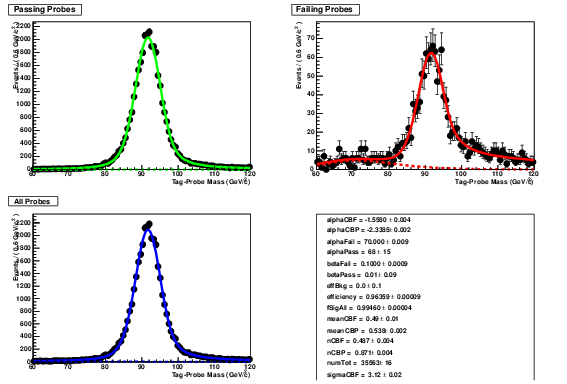
\includegraphics[width=0.8\textwidth]{Systematics/2012data_outputSCToGsfElectron.png}
\caption{Fitting of super-cluster to GSF Electrons for $\epsilon_{RECO}$ calculation.}
\label{fig:2012data_outputSCToGsfElectron}
\end{figure}
%2012data_outputSCToGsfElectron.eps





%\begin{table}[htb]
%\caption{%
%    $\epsilon_{ID} \times \epsilon_{ISO}$ efficiency values from 2012 data and Monte Carlo simulations using the Tag and Probe method by fitting the signal and background.
%}
%\begin{center}
%\begin{tabular}{ | c | c | c | c | c |}
%      \hline
%      $\eta$ coverage & $p_T$ range (GeV) & Efficiency (data) & Efficiency (MC) & Data/MC ratio \\ \hline \hline
%     0.0 $<$ $\eta$ $<$ 0.8 & 10 $<$ $p_T$ $<$ 20 & 22.84\% $\pm$ 10.13\% & 54.53\% $\pm$ 13.17\% & 0.419 $\pm$ 0.212 \\ \hline
%     0.8 $<$ $\eta$ $<$ 1.4 & 10 $<$ $p_T$ $<$ 20 & 37.14\% $\pm$ 0.54\% & 87.12\% $\pm$ 1.68\% & 0.426 $\pm$ 0.010 \\ \hline
%     1.6 $<$ $\eta$ $<$ 2.0 & 10 $<$ $p_T$ $<$ 20 & 56.11\% $\pm$ 0.98\% & 93.84\% $\pm$ 4.98\% & 0.598 $\pm$ 0.033 \\ \hline
%     2.0 $<$ $\eta$ $<$ 2.5 & 10 $<$ $p_T$ $<$ 20 & 56.39\% $\pm$ 1.43\% & 65.03\% $\pm$ 1.81\% & 0.867 $\pm$ 0.033 \\ \hline
%     \hline
%     0.0 $<$ $\eta$ $<$ 0.8 & 20 $<$ $p_T$ $<$ 40 & 96.15\% $\pm$ 0.44\% & 95.88\% $\pm$ 0.30\% & 1.003 $\pm$ 0.006 \\ \hline
%     0.8 $<$ $\eta$ $<$ 1.4 & 20 $<$ $p_T$ $<$ 40 & 94.67\% $\pm$ 3.00\% & 96.75\% $\pm$ 1.88\% & 0.979 $\pm$ 0.036 \\ \hline
%     1.6 $<$ $\eta$ $<$ 2.0 & 20 $<$ $p_T$ $<$ 40 & 95.31\% $\pm$ 0.79\% & 96.29\% $\pm$ 0.24\% & 0.990 $\pm$ 0.009 \\ \hline
%     2.0 $<$ $\eta$ $<$ 2.5 & 20 $<$ $p_T$ $<$ 40 & 95.02\% $\pm$ 0.31\% & 92.90\% $\pm$ 3.64\% & 1.023 $\pm$ 0.040 \\ \hline
%     \hline
%     0.0 $<$ $\eta$ $<$ 0.8 & 40 $<$ $p_T$ $<$ 200 & 97.53\% $\pm$ 0.16\% & 98.22\% $\pm$ 0.05\% & 0.993 $\pm$ 0.002 \\ \hline
%     0.8 $<$ $\eta$ $<$ 1.4 & 40 $<$ $p_T$ $<$ 200 & 98.08\% $\pm$ 0.07\% & 98.63\% $\pm$ 0.05\% & 0.994 $\pm$ 0.001 \\ \hline
%     1.6 $<$ $\eta$ $<$ 2.0 & 40 $<$ $p_T$ $<$ 200 & 96.36\% $\pm$ 0.11\% & 97.47\% $\pm$ 1.31\% & 0.989 $\pm$ 0.013 \\ \hline
%     2.0 $<$ $\eta$ $<$ 2.5 & 40 $<$ $p_T$ $<$ 200 & 95.61\% $\pm$ 0.30\% & 95.67\% $\pm$ 0.12\% & 0.999 $\pm$ 0.003 \\ \hline
%    \end{tabular}
%\end{center}
%\label{tab:tagandprobe_ISO}
%\end{table}


\begin{figure}[htb]
\centering
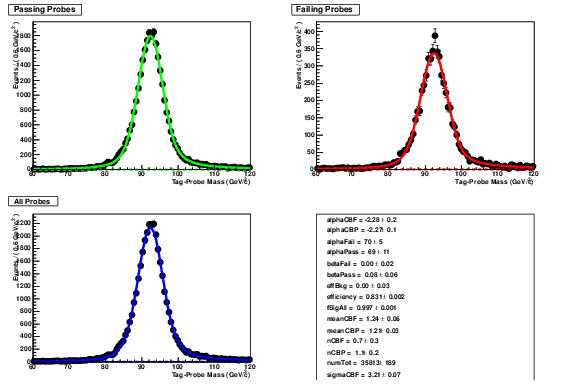
\includegraphics[width=0.8\textwidth]{Systematics/2012data_outputGsfElectronToId.png}
\caption{Fitting of GSF Electrons for $\epsilon_{ISO}$ calculation.}
\label{fig:2012data_outputGsfElectronToId}
\end{figure}
%2012data_outputGsfElectronToId.eps



%\begin{table}[htb]
%\caption{%
%    $\epsilon_{trigger}$ values for Ele8 Leg from 2012 data and Monte Carlo simulations using the Tag and Probe method by counting passing and failing probes.
%}
%\begin{center}

%     \begin{tabular}{ | c | c | c | c | c |}
%      \hline
%      $\eta$ coverage & $p_T$ range (GeV) & Efficiency (data) & Efficiency (MC) & Data/MC ratio \\ \hline \hline
%      0.0 $<$ $\eta$ $<$ 0.8 & 10 $<$ $p_T$ $<$ 20 & 96.03\% $\pm$ 0.37\% & 96.62\% $\pm$ 0.34\% & 0.994 $\pm$ 0.005 \\ \hline
%      0.8 $<$ $\eta$ $<$ 1.4 & 10 $<$ $p_T$ $<$ 20 & 85.50\% $\pm$ 0.64\% & 88.63\% $\pm$ 0.56\% & 0.965 $\pm$ 0.009 \\ \hline
%      1.6 $<$ $\eta$ $<$ 2.0 & 10 $<$ $p_T$ $<$ 20 & 84.15\% $\pm$ 0.99\% & 83.76\% $\pm$ 1.02\% & 1.005 $\pm$ 0.017 \\ \hline
%      2.0 $<$ $\eta$ $<$ 2.5 & 10 $<$ $p_T$ $<$ 20 & 84.80\% $\pm$ 1.04\% & 88.53\% $\pm$ 0.98\% & 0.958 $\pm$ 0.016 \\ \hline
%      \hline
%      0.0 $<$ $\eta$ $<$ 0.8 & 20 $<$ $p_T$ $<$ 40 & 98.19\% $\pm$ 0.05\% & 98.42\% $\pm$ 0.04\% & 0.998 $\pm$ 0.001 \\ \hline
%      0.8 $<$ $\eta$ $<$ 1.4 & 20 $<$ $p_T$ $<$ 40 & 92.99\% $\pm$ 0.11\% & 94.14\% $\pm$ 0.10\% & 0.988 $\pm$ 0.002 \\ \hline
%      1.6 $<$ $\eta$ $<$ 2.0 & 20 $<$ $p_T$ $<$ 40 & 89.07\% $\pm$ 0.20\% & 89.47\% $\pm$ 0.20\% & 0.996 $\pm$ 0.003 \\ \hline
%      2.0 $<$ $\eta$ $<$ 2.5 & 20 $<$ $p_T$ $<$ 40 & 92.59\% $\pm$ 0.19\% & 92.53\% $\pm$ 0.20\% & 1.001 $\pm$ 0.003 \\ \hline
%      \hline
%      0.0 $<$ $\eta$ $<$ 0.8 & 40 $<$ $p_T$ $<$ 200 & 98.81\% $\pm$ 0.04\% & 99.11\% $\pm$ 0.03\% & 0.997 $\pm$ 0.001 \\ \hline
%      0.8 $<$ $\eta$ $<$ 1.4 & 40 $<$ $p_T$ $<$ 200 & 96.92\% $\pm$ 0.07\% & 97.42\% $\pm$ 0.06\% & 0.995 $\pm$ 0.001 \\ \hline
%      1.6 $<$ $\eta$ $<$ 2.0 & 40 $<$ $p_T$ $<$ 200 & 93.22\% $\pm$ 0.15\% & 93.73\% $\pm$ 0.13\% & 0.995 $\pm$ 0.002 \\ \hline
%      2.0 $<$ $\eta$ $<$ 2.5 & 40 $<$ $p_T$ $<$ 200 & 94.74\% $\pm$ 0.15\% & 95.04\% $\pm$ 0.14\% & 0.997 $\pm$ 0.002 \\ \hline
%      \end{tabular}
%\end{center}
%\label{tab:tagandprobe_8}
%\end{table}

%\begin{table}[htb]
%\caption{%
%    $\epsilon_{trigger}$ values for Ele17 Leg from 2012 data and Monte Carlo simulations using the Tag and Probe method by counting passing and failing probes.
%}
%\begin{center}

%    \begin{tabular}{ | c | c | c | c | c |}
%      \hline
%      $\eta$ coverage & $p_T$ range (GeV) & Efficiency (data) & Efficiency (MC) & Data/MC ratio \\ \hline \hline
%      0.0 $<$ $\eta$ $<$ 0.8 & 10 $<$ $p_T$ $<$ 20 & 48.80\% $\pm$ 0.92\% & 57.97\% $\pm$ 0.91\% & 0.842 $\pm$ 0.021 \\ \hline
%      0.8 $<$ $\eta$ $<$ 1.4 & 10 $<$ $p_T$ $<$ 20 & 33.01\% $\pm$ 0.85\% & 46.75\% $\pm$ 0.87\% & 0.706 $\pm$ 0.022 \\ \hline
%      1.6 $<$ $\eta$ $<$ 2.0 & 10 $<$ $p_T$ $<$ 20 & 47.63\% $\pm$ 1.34\% & 47.23\% $\pm$ 1.37\% & 1.008 $\pm$ 0.041 \\ \hline
%      2.0 $<$ $\eta$ $<$ 2.5 & 10 $<$ $p_T$ $<$ 20 & 40.66\% $\pm$ 1.41\% & 50.52\% $\pm$ 1.52\% & 0.805 $\pm$ 0.037 \\ \hline
%      \hline
%      0.0 $<$ $\eta$ $<$ 0.8 & 20 $<$ $p_T$ $<$ 40 & 98.49\% $\pm$ 0.04\% & 98.86\% $\pm$ 0.04\% & 0.996 $\pm$ 0.001 \\ \hline
%      0.8 $<$ $\eta$ $<$ 1.4 & 20 $<$ $p_T$ $<$ 40 & 93.45\% $\pm$ 0.11\% & 94.62\% $\pm$ 0.10\% & 0.988 $\pm$ 0.002 \\ \hline
%      1.6 $<$ $\eta$ $<$ 2.0 & 20 $<$ $p_T$ $<$ 40 & 89.71\% $\pm$ 0.19\% & 89.98\% $\pm$ 0.19\% & 0.997 $\pm$ 0.003 \\ \hline
%      2.0 $<$ $\eta$ $<$ 2.5 & 20 $<$ $p_T$ $<$ 40 & 93.67\% $\pm$ 0.18\% & 93.59\% $\pm$ 0.18\% & 1.001 $\pm$ 0.003 \\ \hline
%      \hline
%      0.0 $<$ $\eta$ $<$ 0.8 & 40 $<$ $p_T$ $<$ 200 & 99.05\% $\pm$ 0.03\% & 99.41\% $\pm$ 0.03\% & 0.996 $\pm$ 0.000 \\ \hline
%      0.8 $<$ $\eta$ $<$ 1.4 & 40 $<$ $p_T$ $<$ 200 & 97.41\% $\pm$ 0.07\% & 97.92\% $\pm$ 0.06\% & 0.995 $\pm$ 0.001 \\ \hline
%      1.6 $<$ $\eta$ $<$ 2.0 & 40 $<$ $p_T$ $<$ 200 & 93.90\% $\pm$ 0.14\% & 94.38\% $\pm$ 0.13\% & 0.995 $\pm$ 0.002 \\ \hline
%      2.0 $<$ $\eta$ $<$ 2.5 & 40 $<$ $p_T$ $<$ 200 & 95.93\% $\pm$ 0.13\% & 96.17\% $\pm$ 0.12\% & 0.998 $\pm$ 0.002 \\ \hline
%    \end{tabular}
%\end{center}
%\label{tab:tagandprobe_17}
%\end{table}



%%%%%%%%%%%%%%%%%%%%%%%%%%%%%%%%%%%%%%%%%%%%%%%%%

\subsection{Jet Reconstruction}
\label{JESsystematics}

There are two components of the uncertainty on jets.  One is the jet energy scale (JES) and the other is the resolution.  The resolution uncertainty is negligible compared to other uncertainties, but the JES does make a measurable effect.  The uncertainty on the JES is computed by shifting the $p_T$ of the jets $\pm 1 \sigma$ with respect to the measured JES.  This shifting of the jet $p_T$ changes the $p_T$ spectrum of the jet which effects the dijet invariant mass, and ultimately the reconstructed Higgs boson mass.  Table ~\ref{tab:JES} shows the uncertainty for a range of generated Higgs mass samples. The effect of jet resolution uncertainty on the signal was done by smearing a sub-sample of jets in a sample and looking at the difference between smeared and non smeared events. The effect was negligible.  The background is evaluated from data so there should not be a significant effect on those events.


\begin{table}[htb]
\caption{%
    Jet energy scale (JES) uncertainty for a variety of Higgs boson masses.
}
\begin{center}

    \begin{tabular}{ | c | c | c |}
      \hline
      $M_H$ GeV & JES -1$\sigma$ & JES +1$\sigma$ \\ \hline \hline
      230  & -4.17\% & 4.26\% \\
      300  & -1.30\% & 1.33\% \\
      400  & -1.20\% & 1.23\% \\ 
      600  & 0.86\%  & 0.79\% \\
      800  & 1.10\%  & 1.08\% \\
      1000 & 1.21\%  & 1.16\% \\ \hline
      
    \end{tabular}
\end{center}
\label{tab:JES}
\end{table}



%%%%%%%%%%%%%%%%%%%%%%%%%%%%%%%%%%%%%%%%%%%%%%%%%

\subsection{b-Tagging}
Scale factors between data and simulation have been measured for events with b-jets in bins as a function of $p_T$ and $\eta$.  This solves the problem that b-jets are more correctly identified in Monte Carlo simulation than they are in data.  Also, a mis-tag rate scale factor is calculated when light-quark and gluon jets are tagged as jets from the hadronization of heavy quarks.  For the systematic effects, both the scale factor for tagging ($SF_b$) and scale factor for mis-tags ($SF_{mis-tag}$) are varied up and down by the uncertainty related to each SF. In the analysis, the exact systematic uncertainty (computed as a function of the Higgs mass) is applied.


%%%%%%%%%%%%%%%%%%%%%%%%%%%%%%%%%%%%%%%%%%%%%%%%%%%%%%%%%%%%%%%%%%%%%%%%%

\subsection{MET uncertainty}

When looking at MET uncertainty, the bulk of the effect comes from our knowledge of the rest of the event, primarily jet energy reconstruction and pile-up.  As both of these uncertainties are treated already, much of the MET uncertainty is already taken into account.  In signal and Z+jets background there is no real MET, but it is expected to be seen in $\Pqt \Paqt$ events.  The uncertainty is found by subtracting the $\Pqt \Paqt$ MC contribution from both data and simulation, and then looking at the differences between the two. In addition, we look at how much of the MET re-scaling described in section~\ref{sec:METsection} affects the signal selection efficiency.  This is done by counting the number of signal events that cross the final MET cut that we use.  This equates to about $\sim 0.5$\% uncertainty on the final efficiency.

%%%%%%%%%%%%%%%%%%%%%%%%%%%%%%%%%%%%%%%%%%%%%%%%%
\subsection{Pile-up}
\label{sec:pileupSystematics}
The number of true interactions per bunch crossing in the simulated samples is re-weighed to match the distributions in data. The uncertainty on the measurement of the amount of pile-ups in data is applied to this analysis. This can modify the signal efficiency in primarily two ways.  First, there are additional particles in the jets which will change the reconstructed four-momentum.  Second, this will introduce a bias in the lepton isolation variables and lower the efficiency in the lepton requirements. 
  This uncertainty is studied by re-estimating the number of true interactions in data with different values of minimum-bias cross section as input.  We use 65.84~mb and 72.77~mb as recommended by the CMS pile-up group~\cite{pileupsys}, which corresponds to a $\pm 5\%$ difference with respect to the central value 69.30~mb. The re-estimated distributions and the central value are compared in Figure~\ref{fig:shiftedDataPileup}. The number of true interactions are re-weighted in the MC to match the shifted distributions in data and then we recompute the signal efficiency. This leads to a change in the signal efficiency $< 1\%$ for the 0- and 1-btag categories, and about 2\% for the 2-btag category, for $\MH < 650 GeV$, approximately independent of lepton channel.  These numbers and additional details can be seen in Appendix~\ref{sec:appsyst}.

\begin{figure}[bh]
\centering
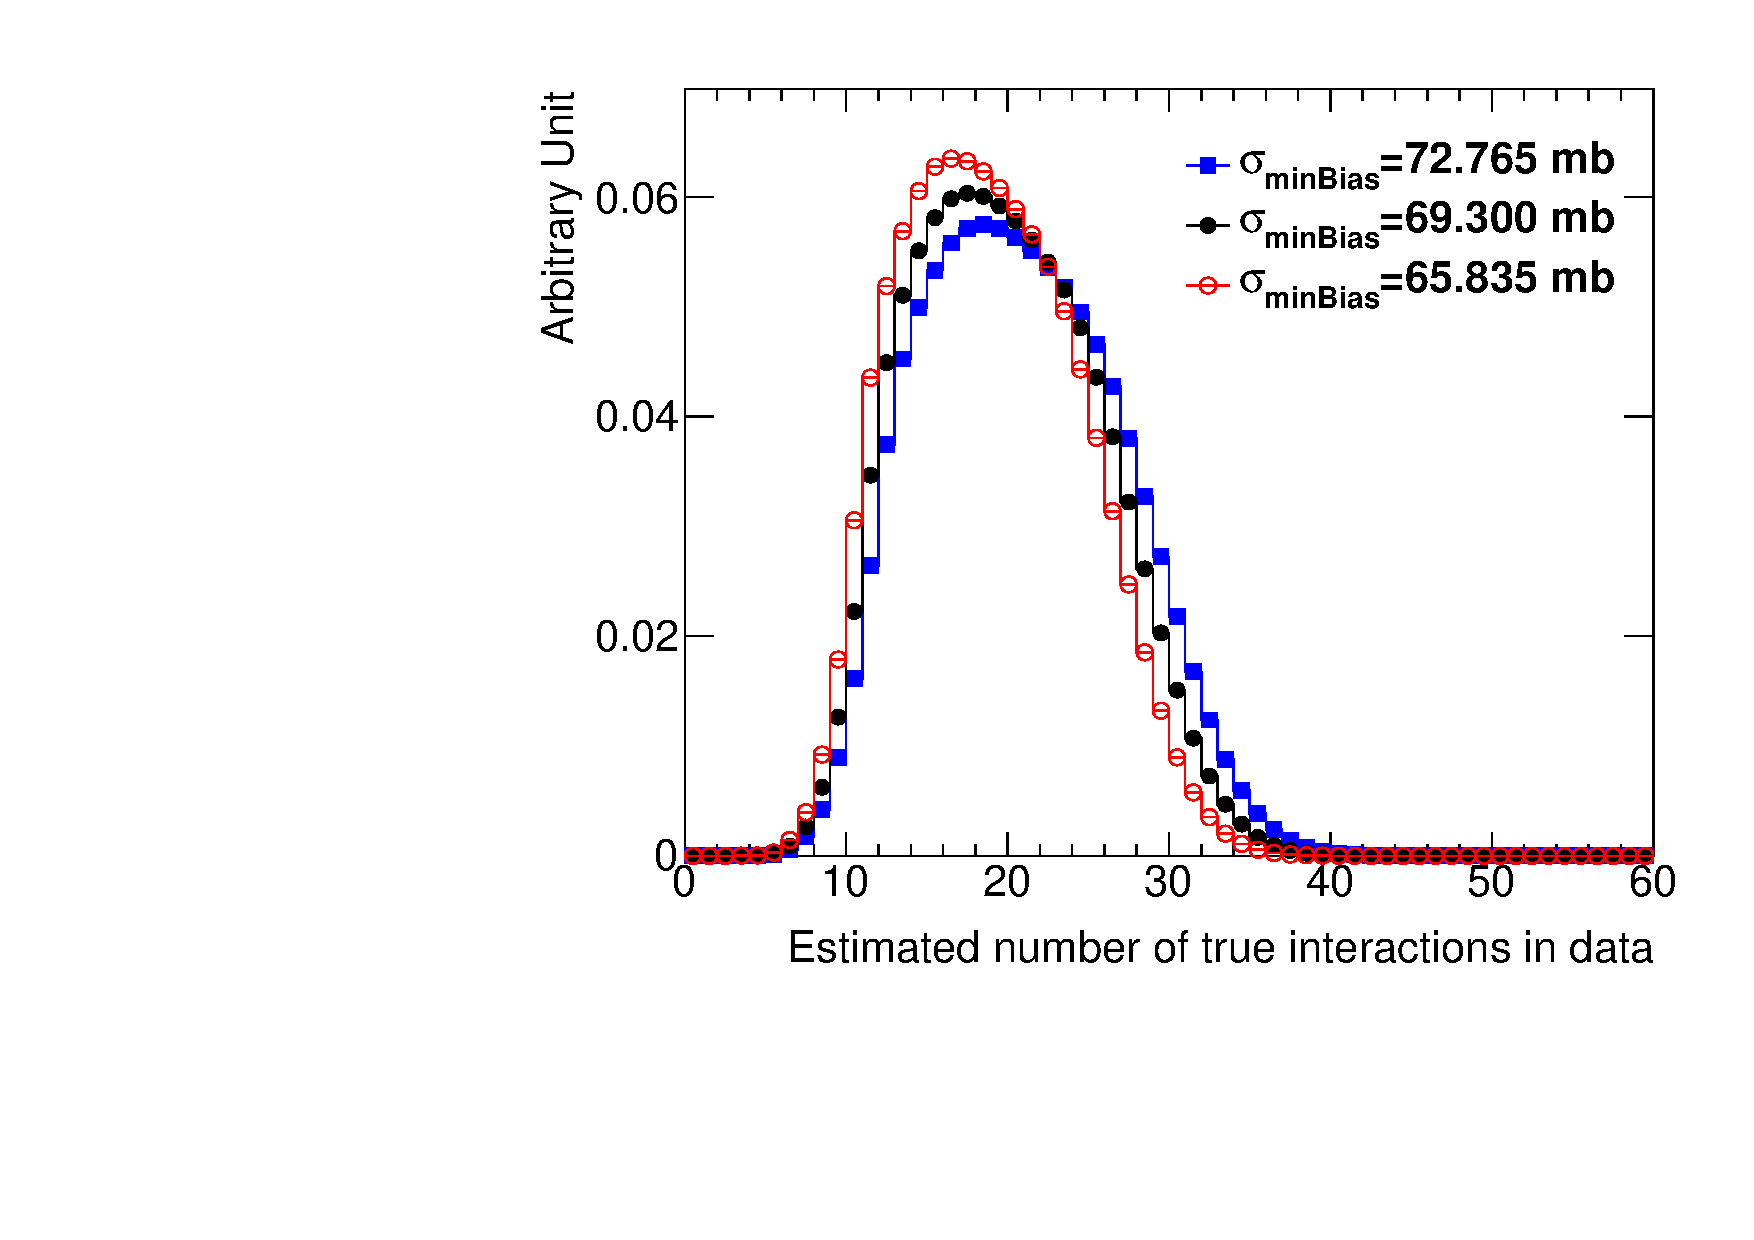
\includegraphics[width=0.49\textwidth]{plots/data_pileup.pdf}
\caption{Estimated number of true interactions in 2012 data, assuming different values of minimum-bias cross section. The central value is 69.3~mb (solid circles).}
\label{fig:shiftedDataPileup}
\end{figure}

%%%%%%%%%%%%%%%%%%%%%%%%%%%%%%%%%%%%%%%%%%%%%%%%%

\subsection{Production mechanism}

The expected kinematics of the Higgs production is subject to uncertainties due to limited knowledge of  the underlying parton distribution functions (PDFs) as well as the shortcomings in the theoretical prediction (missing higher orders in the perturbation series). These uncertainties are propagated to an uncertainty on the selection acceptance and efficiency. Their additional effect on the Higgs production cross section is discussed in a separate section below.

The PDF uncertainties are evaluated according to the PDF4LHC recommendations~\cite{pdf4lhc}, by computing the selection efficiency for the following PDF sets: cteq66~\cite{cteq}, MSTW2008NLO~\cite{MSTW} and  NNPDF2.1~\cite{NNPDF} and their error sets. The envelope of the various PDF sets is used as the total uncertainty, as recommended, and amounts to 1-4\%. The uncertainty noticeably increases for very high Higgs masses. A summary of systematic uncertainties on the signal acceptance following PDF4LHC recommendations can be found in table~\ref{tab:pdf}.

\def\arraystretch{1.7}
\begin{table*}[hb]
\caption{Systematic uncertainties on the signal acceptance following PDF4LHC recommendations.}
\label{tab:pdf}
\begin{center}
\small
\begin{tabular}{|l|ccccc|}
\cline{2-6}
\multicolumn{1}{c|}{} & \multicolumn{5}{c|}{$\MH$ (GeV)} \\ \hline
PDF         & 200               & 400               & 600               & 800               & 1000             \\ \hline
CTEQ66      & $^{+0.6}_{-0.7}$  & $^{+0.8}_{-1.0}$  & $^{+0.8}_{-1.1}$  & $^{+1.5}_{-2.0}$  & $^{+2.6}_{-3.2}$ \\
MSTW2008NLO & $^{-0.2}_{-0.5}$  & $^{+0.6}_{+0.2}$  & $^{+0.8}_{+0.4}$  & $^{+1.5}_{+0.7}$  & $^{+2.5}_{+1.2}$ \\
NNPDF2.1    & $^{+0.8}_{+0.2}$  & $^{+1.4}_{+0.75}$ & $^{+1.5}_{+0.9}$  & $^{+2.7}_{+1.4}$  & $^{+4.3}_{-2.4}$ \\ \hline
Total       & $^{+0.8}_{-0.7}$  & $^{+1.4}_{-0.8}$  & $^{+1.5}_{-1.1}$  & $^{+2.7}_{-2.0}$  & $^{+4.3}_{-3.2}$ \\ \hline
\end{tabular}
\end{center}
\end{table*}
\def\arraystretch{1}

Additional uncertainties arise due to the theoretically calculated Higgs signal shape. The shape uncertainty is evaluated in the recommended way for the Higgs decaying into a pair of Z boson, correctly accounting for the correct line-shape (i.e. re-weighting of the given shape in POWHEG) which also accounts for interference effects. The full description of the re-weighting and uncertainty method is given in~\cite{4l} and provides an uncertainty that contributes in two ways. Due to the mass-dependence of the selection efficiency, the total signal efficiency is affected by the line-shape. 
%Efficiency curves for the nominal and alternative line shapes are shown in figure~\ref{fig:shapeff}.
This uncertainty is negligible below 400 GeV{} and rises to $\sim3\%$ at 600 GeV{}, with only small dependence on btag category.
%%%%%%%%%%%%
%\begin{figure}[htb]
%\begin{center}
%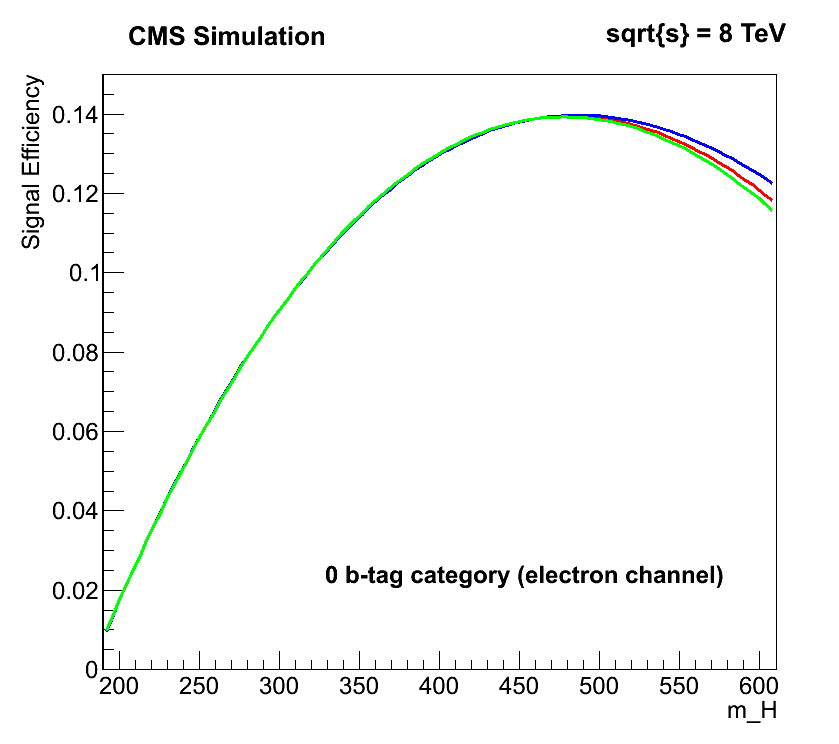
\includegraphics[width=0.3\textwidth]{plots/effFitLsErrors_ELE_0btag.png}
%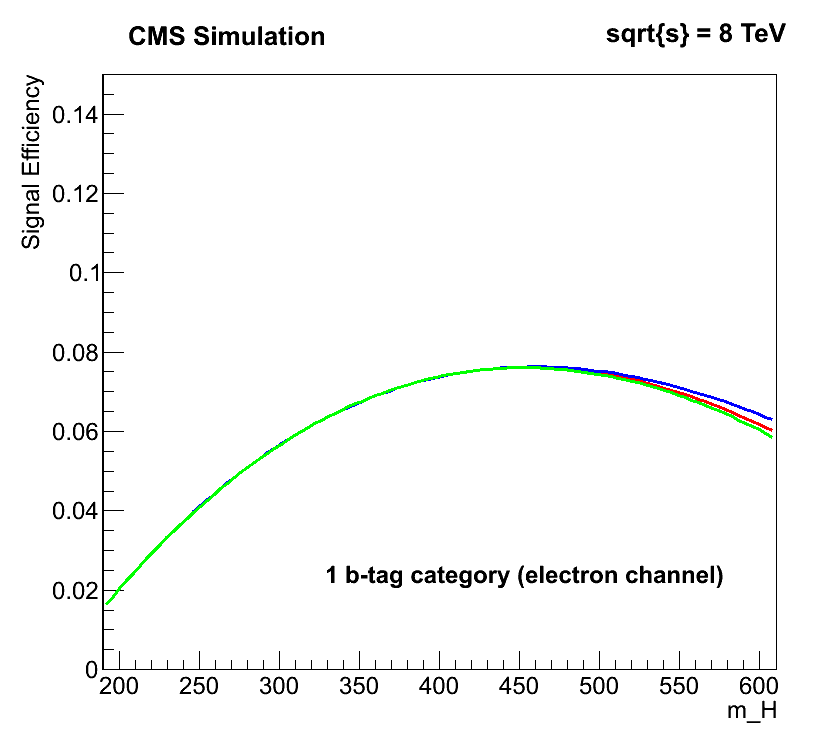
\includegraphics[width=0.3\textwidth]{plots/effFitLsErrors_ELE_1btag.png}
%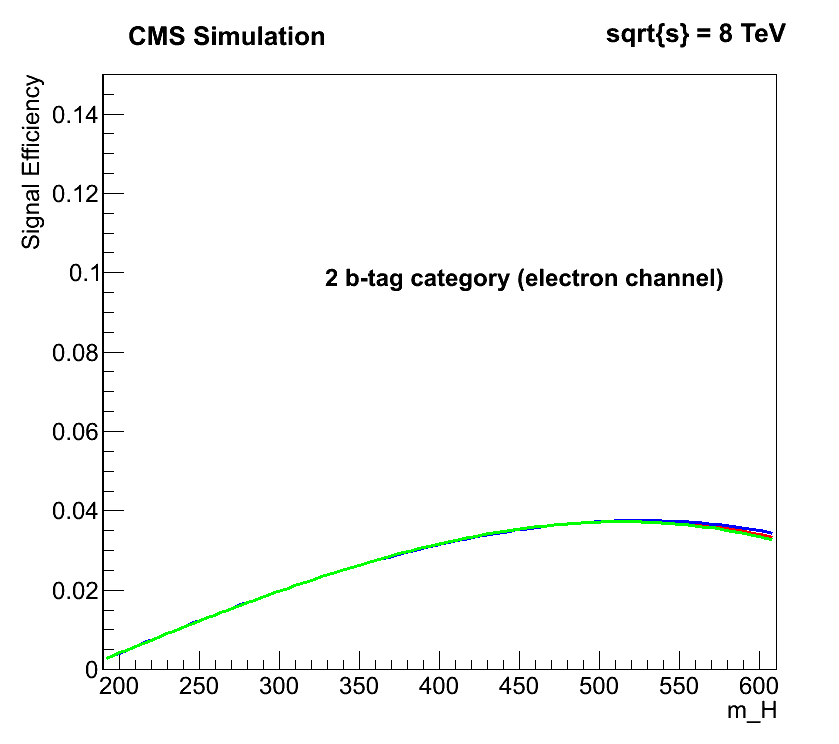
\includegraphics[width=0.3\textwidth]{plots/effFitLsErrors_ELE_2btag.png}\\
%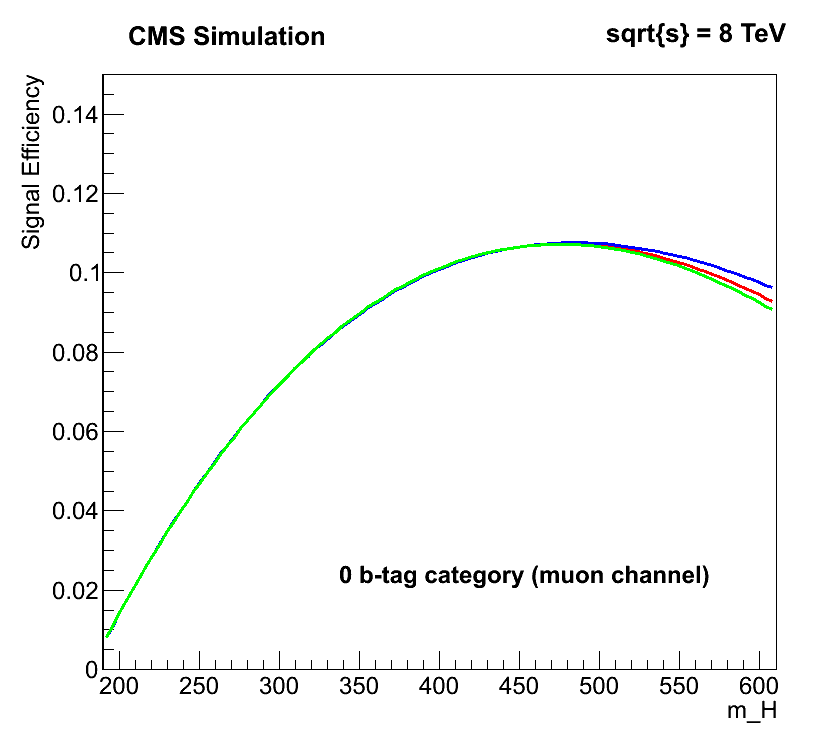
\includegraphics[width=0.3\textwidth]{plots/effFitLsErrors_MU_0btag.png}
%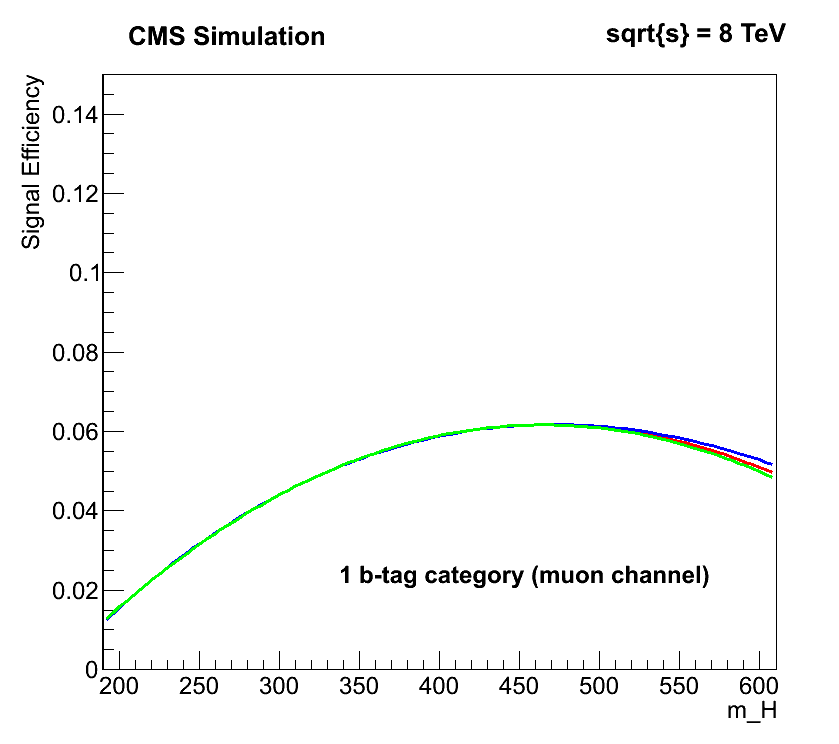
\includegraphics[width=0.3\textwidth]{plots/effFitLsErrors_MU_1btag.png}
%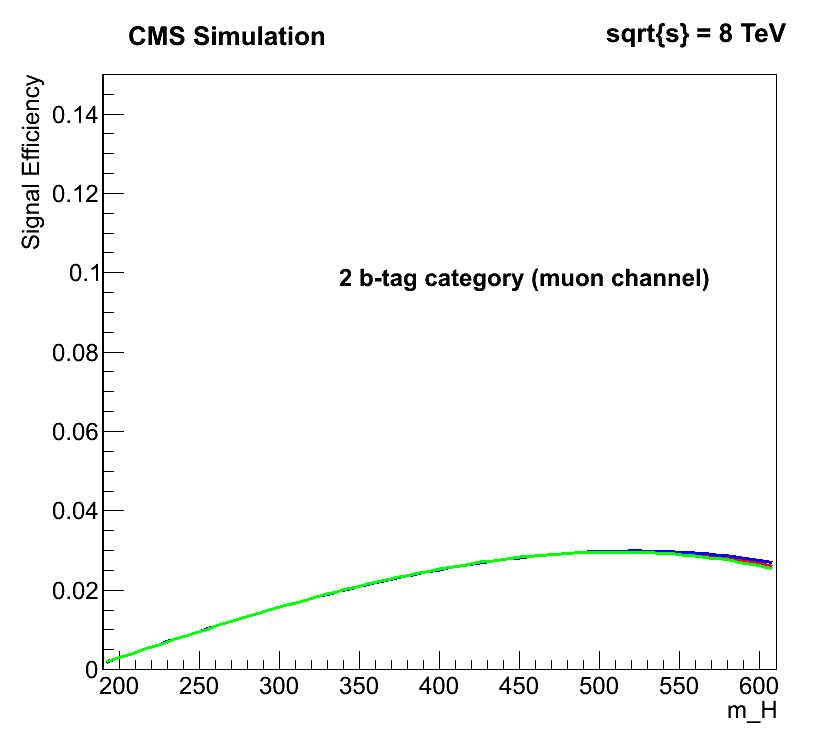
\includegraphics[width=0.3\textwidth]{plots/effFitLsErrors_MU_2btag.png}
%\caption{Signal selection efficiency for the nominal line shape (read) and alternative shapes (green/blue) for electrons (top) and muons (bottom) for 0/1/2 btags (left/middle/right).}
%\label{fig:shapeff}
%\end{center}
%\end{figure}
%%%%%%%%%%%%


The line-shape used in the CLs procedure is re-extracted with the alternative line-shape models (Figure~\ref{fig:lineshape}~(left)). The tail caused by mismatched jets is not affected at all, as it is a random mixture of events, averaging out any shifts from the uncertainty. The core of the signal distribution is only weakly affected by the uncertainty. In the worst case (the highest mass we consider), the peak-position shifts by $\sim2 GeV$ (compared to a sigma of 60 GeV{}) and the sigma changes by $\sim1 GeV$. Due to the minuscule effect of this uncertainty, it is not propagated further.

%%%%%%%%%%%%
\begin{figure}[htb]
\begin{center}
\centerline{
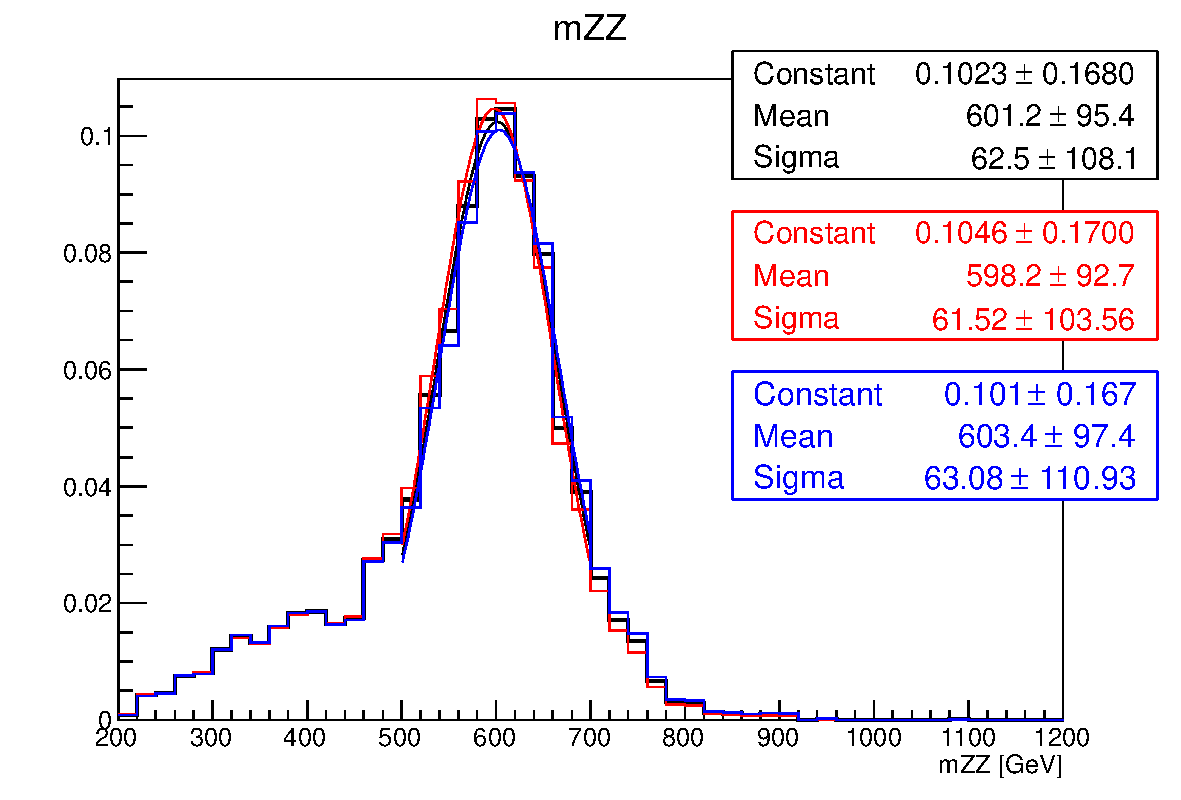
\includegraphics[width=0.56\textwidth]{plots/lineshapeunc.pdf}
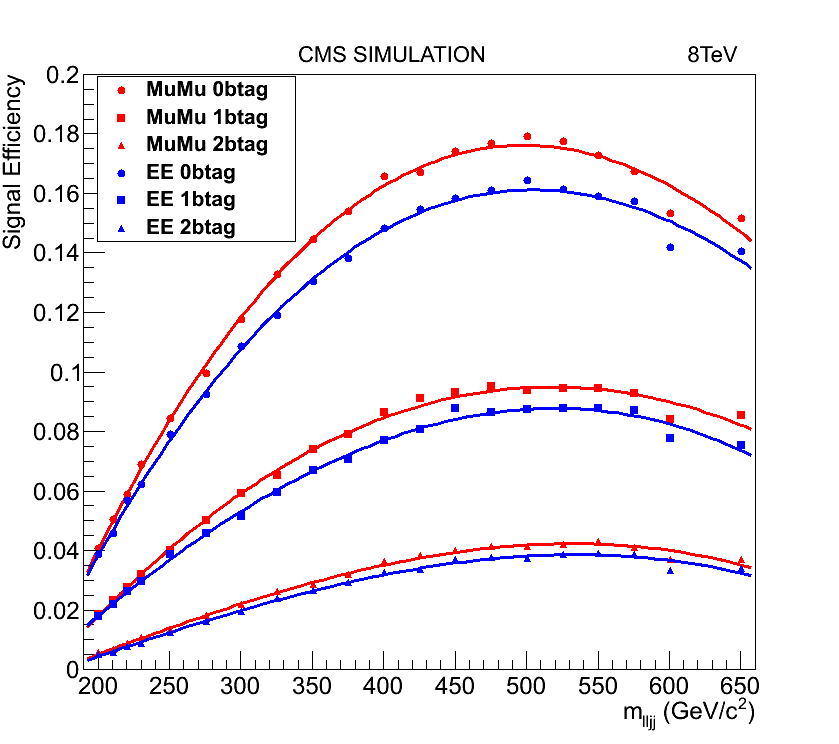
\includegraphics[width=0.44\textwidth]{plots/all_signal_effs.png}
}
\caption{Left: reconstructed $\MH = 600 GeV$ Higgs signal (area normalized) with the nominal line-shape (black) and systematic variations (blue/red). Gaussian fits to the core of the distribution are overlaid. Right: parameterization of the signal efficiencies, as function of the Higgs mass hypothesis, in the three btag categories, and the muon and electron channels.
}
\label{fig:lineshape}
\end{center}
\end{figure}
%%%%%%%%%%%%

%%%%%%%%%%%%%%%%%%%%%%%%%%%%%%%%%%%%%%%%%%%%%%%%%


\subsection{Luminosity uncertainty}

The latest recommendation for the 2012 data sets is the uncertainty on LHC luminosity of 4.4$\%$~\cite{CMS-PAS-LUM-12-001}.

\subsection*{Higgs cross section and branching fractions}

The Higgs production cross section uncertainty depends on production mechanisms, either gluon fusion or vector boson fusion (VBF). However, since the gluon fusion mechanism dominates, it drives the total uncertainty.  We use $gg$ and VBF errors separately and for each mass point according to Yellow Report prescription~\cite{LHCHiggsCrossSectionWorkingGroup:2012ti}. The total weighted error is in the range 13--15\%. This uncertainty does not affect the absolute cross section measurement.


%%%%%%%%%%%%%%%%%%%%%%%%%%%%%%%%%%%%%%%%%%%%%%%%%















%%%%%%%%%%%%%%%%%%%%%%%%%%%%%%%%%%%%%%%%%%%%%%%%%
\section{Background systematic uncertainties}

The main systematic uncertainties on the background normalization and shape are summarized in Table~\ref{table-syst-bg}.


\begin{table*}[htb]
\caption{
Summary of systematic uncertainties on the normalization and shape of the background determination.
}
\label{table-syst-bg}
%\vspace*{\medskipamount}
\begin{center}
\small
\begin{tabular}{|l|c|c|}
\hline
Source                           &   Normalization   &   Shape  \\ \hline \hline
Muon trigger \& ID               &  2.7\%            &          \\
Muon momentum scale              &  0.1\%            &          \\
Electron trigger \& ID           &  2.0\%            &          \\
Electron energy scale            &  0.5\%            &          \\
Jet energy scale                 &  5.5\%            &   0-4\%  \\ 
\hline
$b$-tagging efficiency SF 0-tag  & +0.4\%            &          \\ 
$b$-tagging efficiency SF 1-tag  & -0.8\%            &          \\ 
$b$-tagging efficiency SF 2-tag  & -4.5\%            &          \\ 
\hline
Mis-tag SF 0-tag                  & -1.9\%            &          \\ 
Mis-tag SF 1-tag                  & +7.8\%            &          \\ 
Mis-tag SF 2-tag                  & +6.2\%            &          \\ 
\hline
MET                              &  0.3\%            &          \\ 
Pile-up                          &  0.1\%            &          \\
$\pt^{\ell\ell jj}$ re-weighting    &  0.8\%            &   0-3\%  \\
Diboson cross section            &  15\%             &          \\
Luminosity                       &  4.4\%           &          \\ \hline 
Residual difference              &                   &  0-15\% (0-btag) \\
data-background in               &                   &  0-30\% (1-btag) \\
control region                   &                   &  0-40\% (2-btag) \\
\hline 
\end{tabular} 
\end{center} 
\end{table*} 

\subsection{Background normalization uncertainties}

Lepton trigger and reconstruction uncertainties yield a 2\% variation in the
normalization of the $\mlljj$ spectrum. Uncertainties on the muon momentum scale,
electron energy scale, pile-up re-weighting and the MET re-scaling procedure have a negligible impact. JES uncertainty 
causes an uncertainty on the normalization of 5.5\%. The uncertainty on the scale factors for the b-tagging efficiency has an effect on the normalization of 0.4\%, 0.8\% and 4.5\% for the the 0-, 1- and 2-btag categories respectively. The uncertainty on the b-tagging mis-tag rates introduces an uncertainty in the normalization of 1.9\%, 7.8\% and 6.2\% for the the 0-, 1- and 2-btag categories respectively.






\subsection{Background shape uncertainties}

The impact on the $\mlljj$ distributions of the uncertainties affecting the shape is displayed in Figures~\ref{fig:sysshape} and~\ref{fig:sysshape2d}. Jet energy scale causes a $\mlljj$-dependent uncertainty varying from almost 0 at low mass, up to 4\% at 600 GeV.

To estimate the impact of the $\pt^{\ell\ell jj}$ correction, we compare the $\mlljj$ Z+jets background distributions with and without the correction. A mass-dependent systematic uncertainty is obtained as the difference of those distributions and goes up to 3\% at high $\mlljj$ values.

Residual differences in the $\mlljj$ distributions between the data and the background in the $M_{jj}$ sideband control region are taken as an additional mass-dependent systematic uncertainty. Those residual differences are plotted in Figure~\ref{fig:sysshaperes}~(top). In order to smooth out the fluctuations, a linear variation as shown in the figure is used to incorporate this effect into alternative templates for the background prediction. The resulting alternative templates, around the nominal template, are shown in Figure~\ref{fig:sysshaperes}~middle and bottom, for the electron and muon channels respectively. 



\begin{figure}[htb]
\begin{center}
\centerline{
%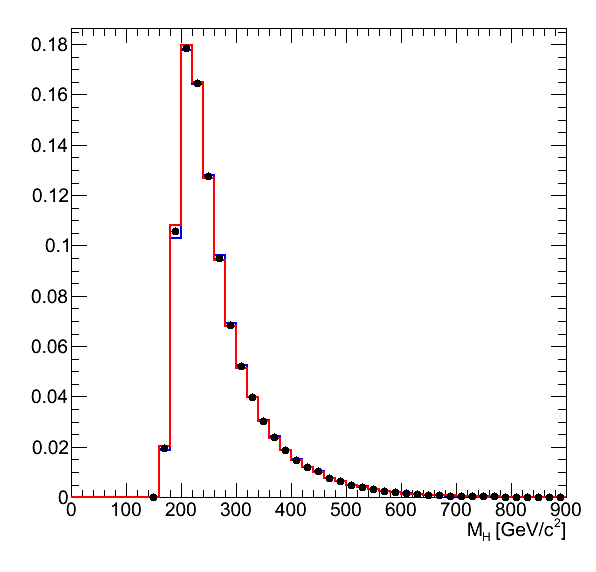
\includegraphics[width=0.33\textwidth]{plots/dy_es.png}
%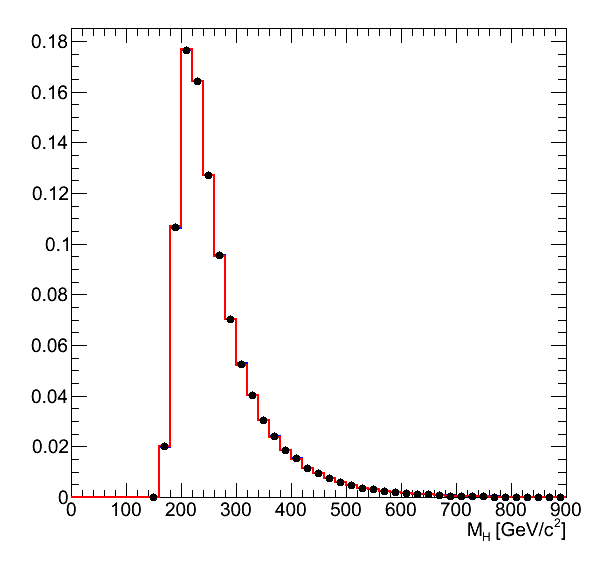
\includegraphics[width=0.33\textwidth]{plots/dy_ms.png}
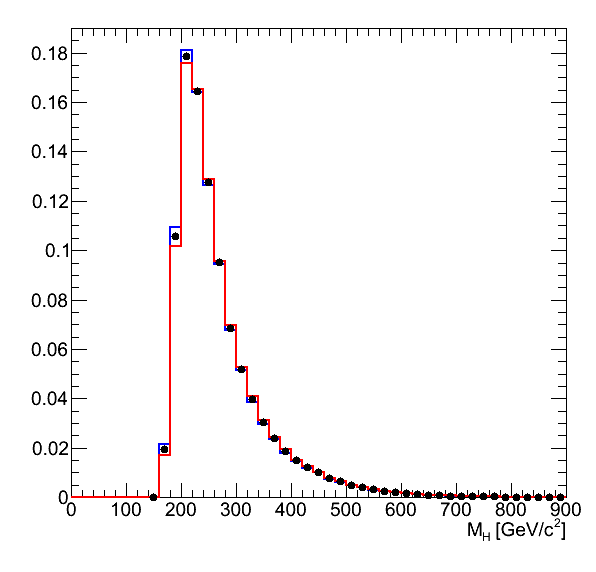
\includegraphics[width=0.49\textwidth]{plots/dy_jse.png}
%}
%\centerline{
%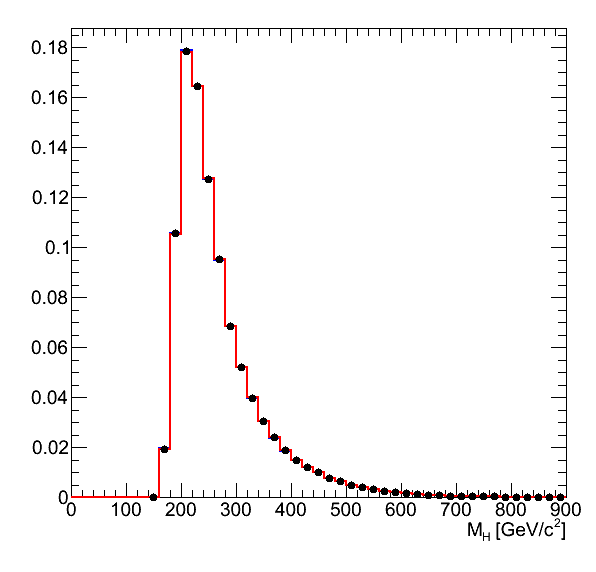
\includegraphics[width=0.33\textwidth]{plots/dy_pue.png}
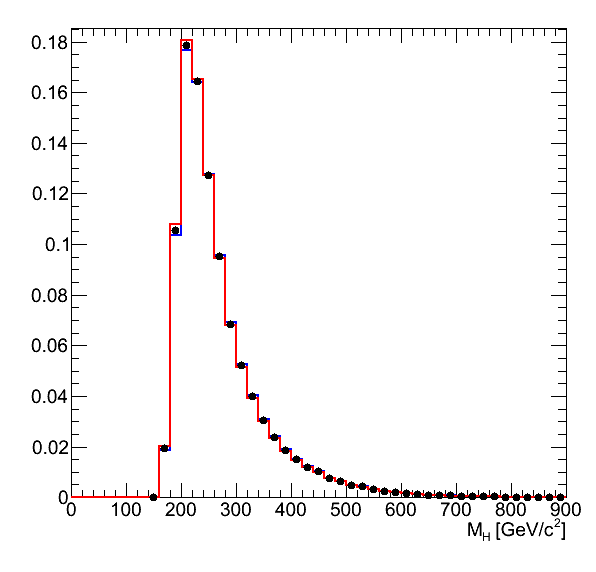
\includegraphics[width=0.49\textwidth]{plots/dy_pthe.png}
% 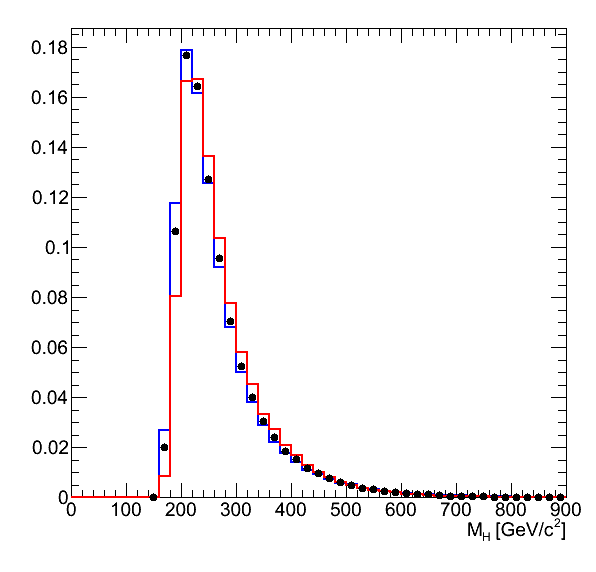
\includegraphics[width=0.33\textwidth]{plots/dy_shm.png}
}
\caption{Shape variation of the $\mlljj$ distribution for Z+jets simulated
events when varying the systematic uncertainties: (left) jet energy scale,
(right) $\pt^{\ell\ell jj}$-based re-weighting. Black dots denote
the reference shapes. Red and blue histograms indicate the up and down variations
of the corresponding systematic uncertainties.
}
\label{fig:sysshape}
\end{center}
\end{figure}

\begin{figure}[htb]
\begin{center}
\centerline{
%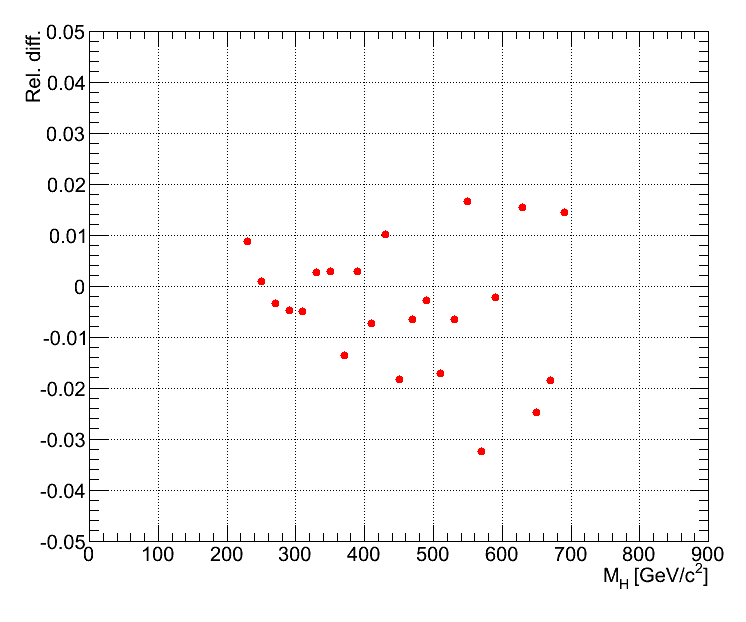
\includegraphics[width=0.33\textwidth]{plots/dy2_es.png}
%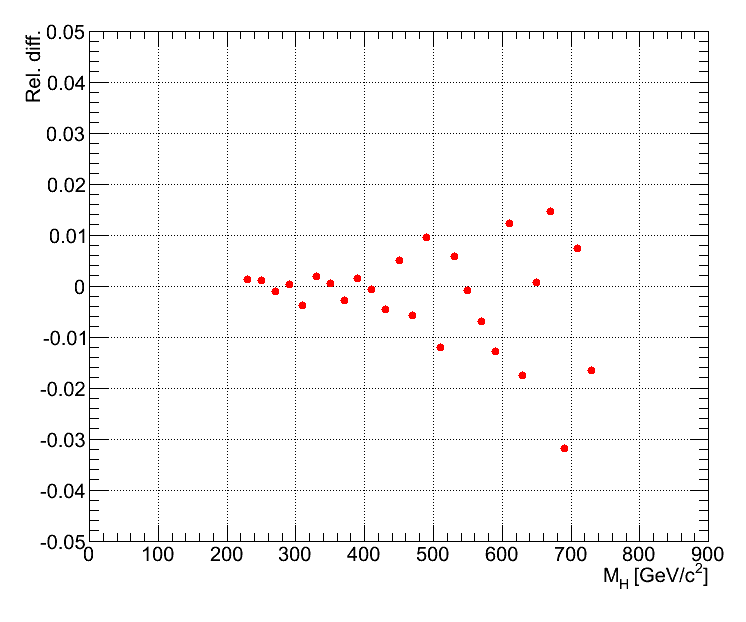
\includegraphics[width=0.33\textwidth]{plots/dy2_ms.png}
%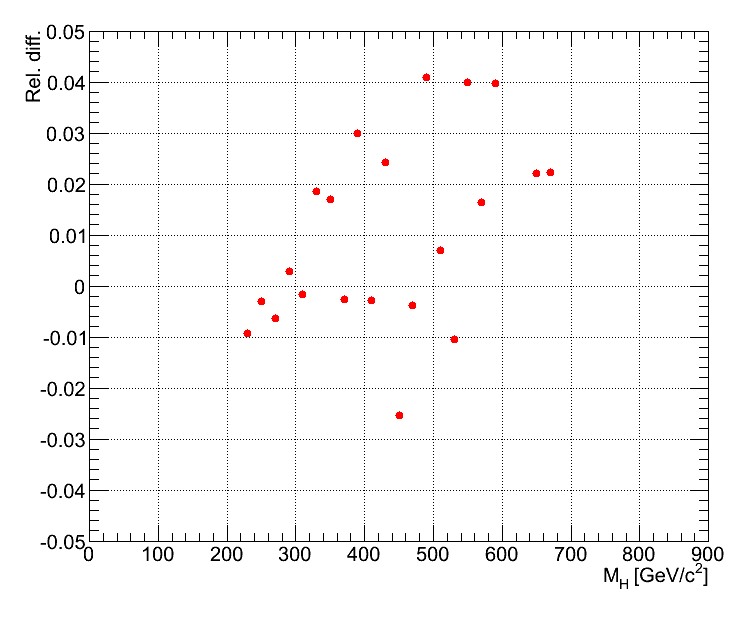
\includegraphics[width=0.49\textwidth]{plots/dy2_jse.png}
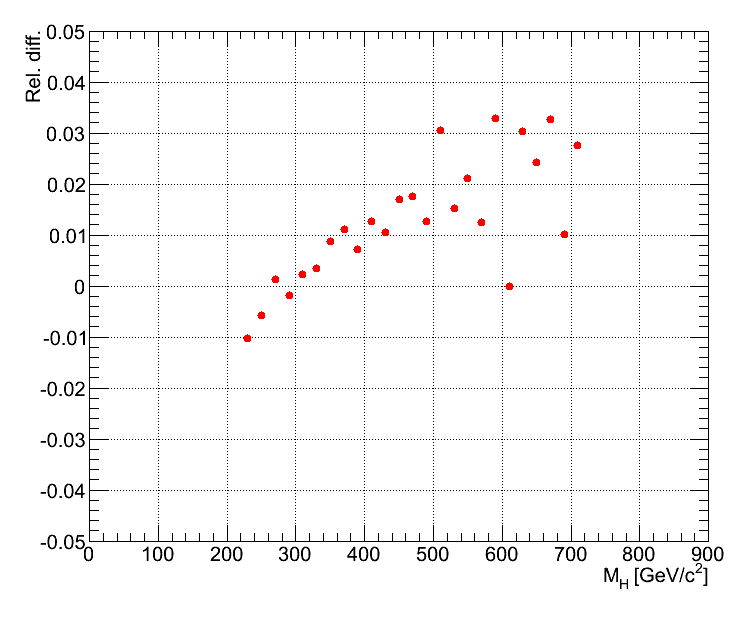
\includegraphics[width=0.49\textwidth]{plots/dy2_jsm.png}
%}
%\centerline{
%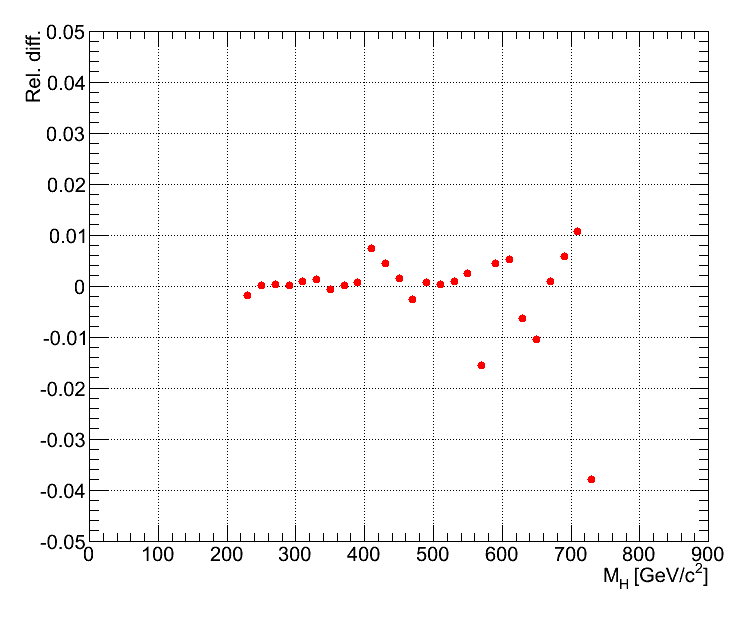
\includegraphics[width=0.33\textwidth]{plots/dy2_pue.png}
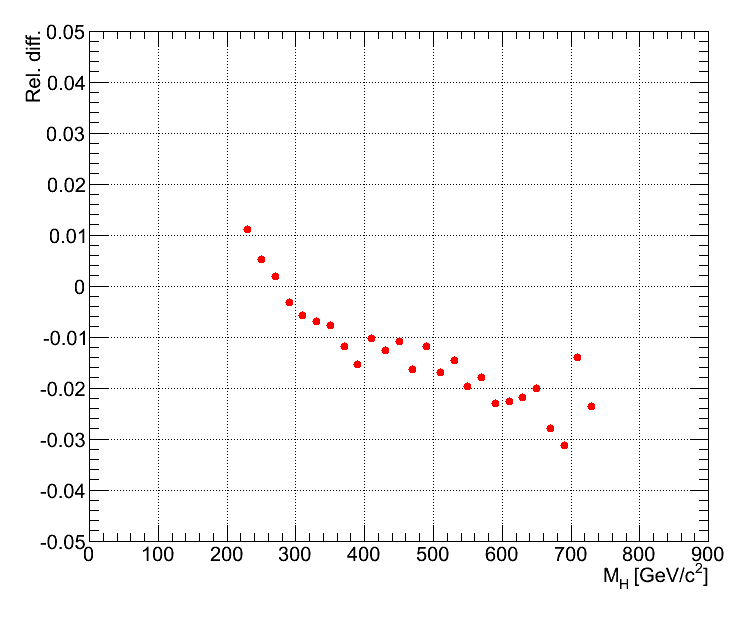
\includegraphics[width=0.49\textwidth]{plots/dy2_pthe.png}
% 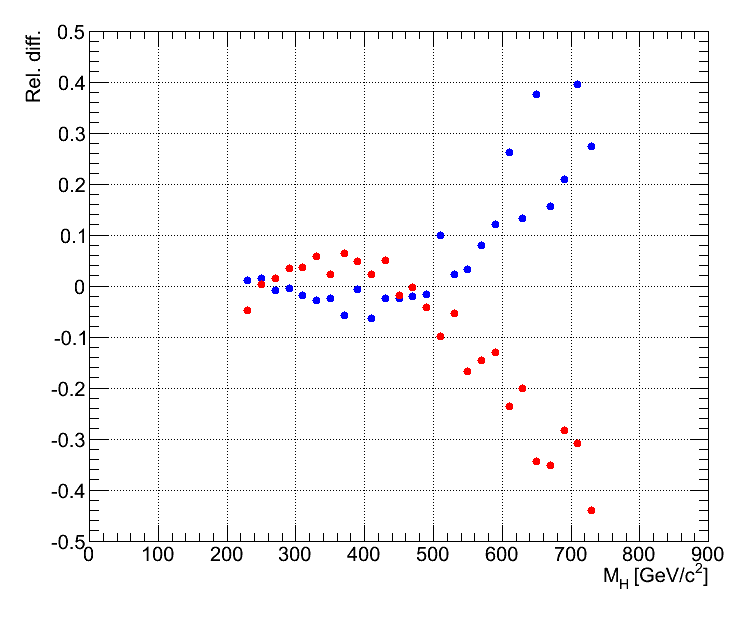
\includegraphics[width=0.33\textwidth]{plots/dy2_shm.png}
}
\caption{Relative difference on the shape of the $\mlljj$ distribution for Z+jets simulated
events when varying the systematic uncertainties: (left) jet energy scale,
(right) $\pt^{\ell\ell jj}$-based re-weighting.
}
\label{fig:sysshape2d}
\end{center}
\end{figure}

\begin{figure}[htb]
\begin{center}
\centerline{
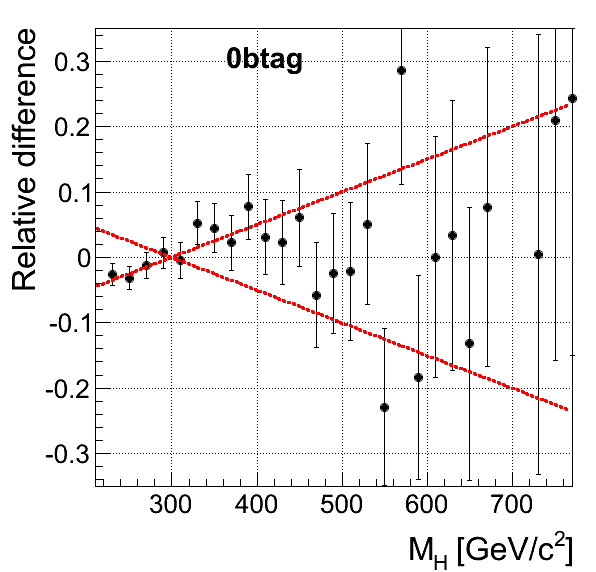
\includegraphics[width=0.33\textwidth]{plots/Diff_SBresidual_0btag.png}
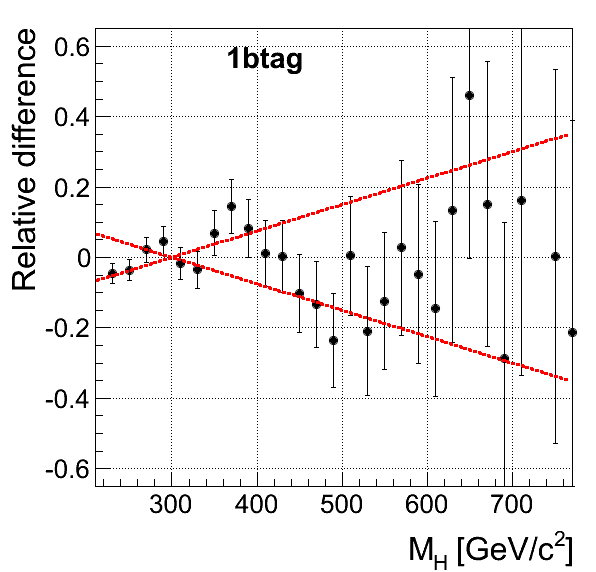
\includegraphics[width=0.33\textwidth]{plots/Diff_SBresidual_1btag.png}
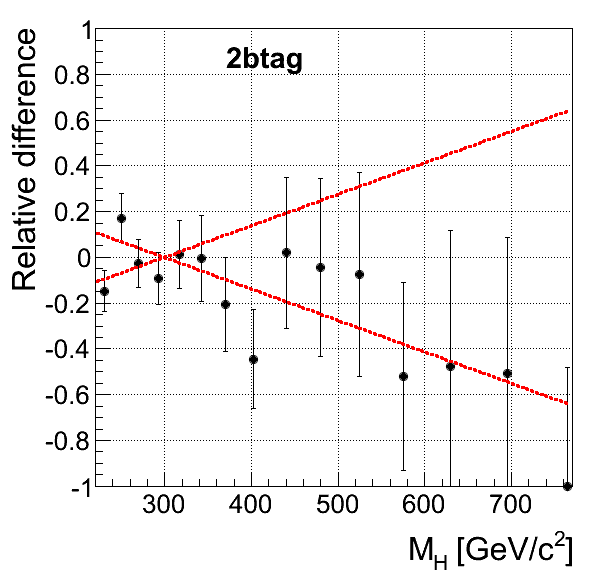
\includegraphics[width=0.33\textwidth]{plots/Diff_SBresidual_2btag.png}
}
\centerline{
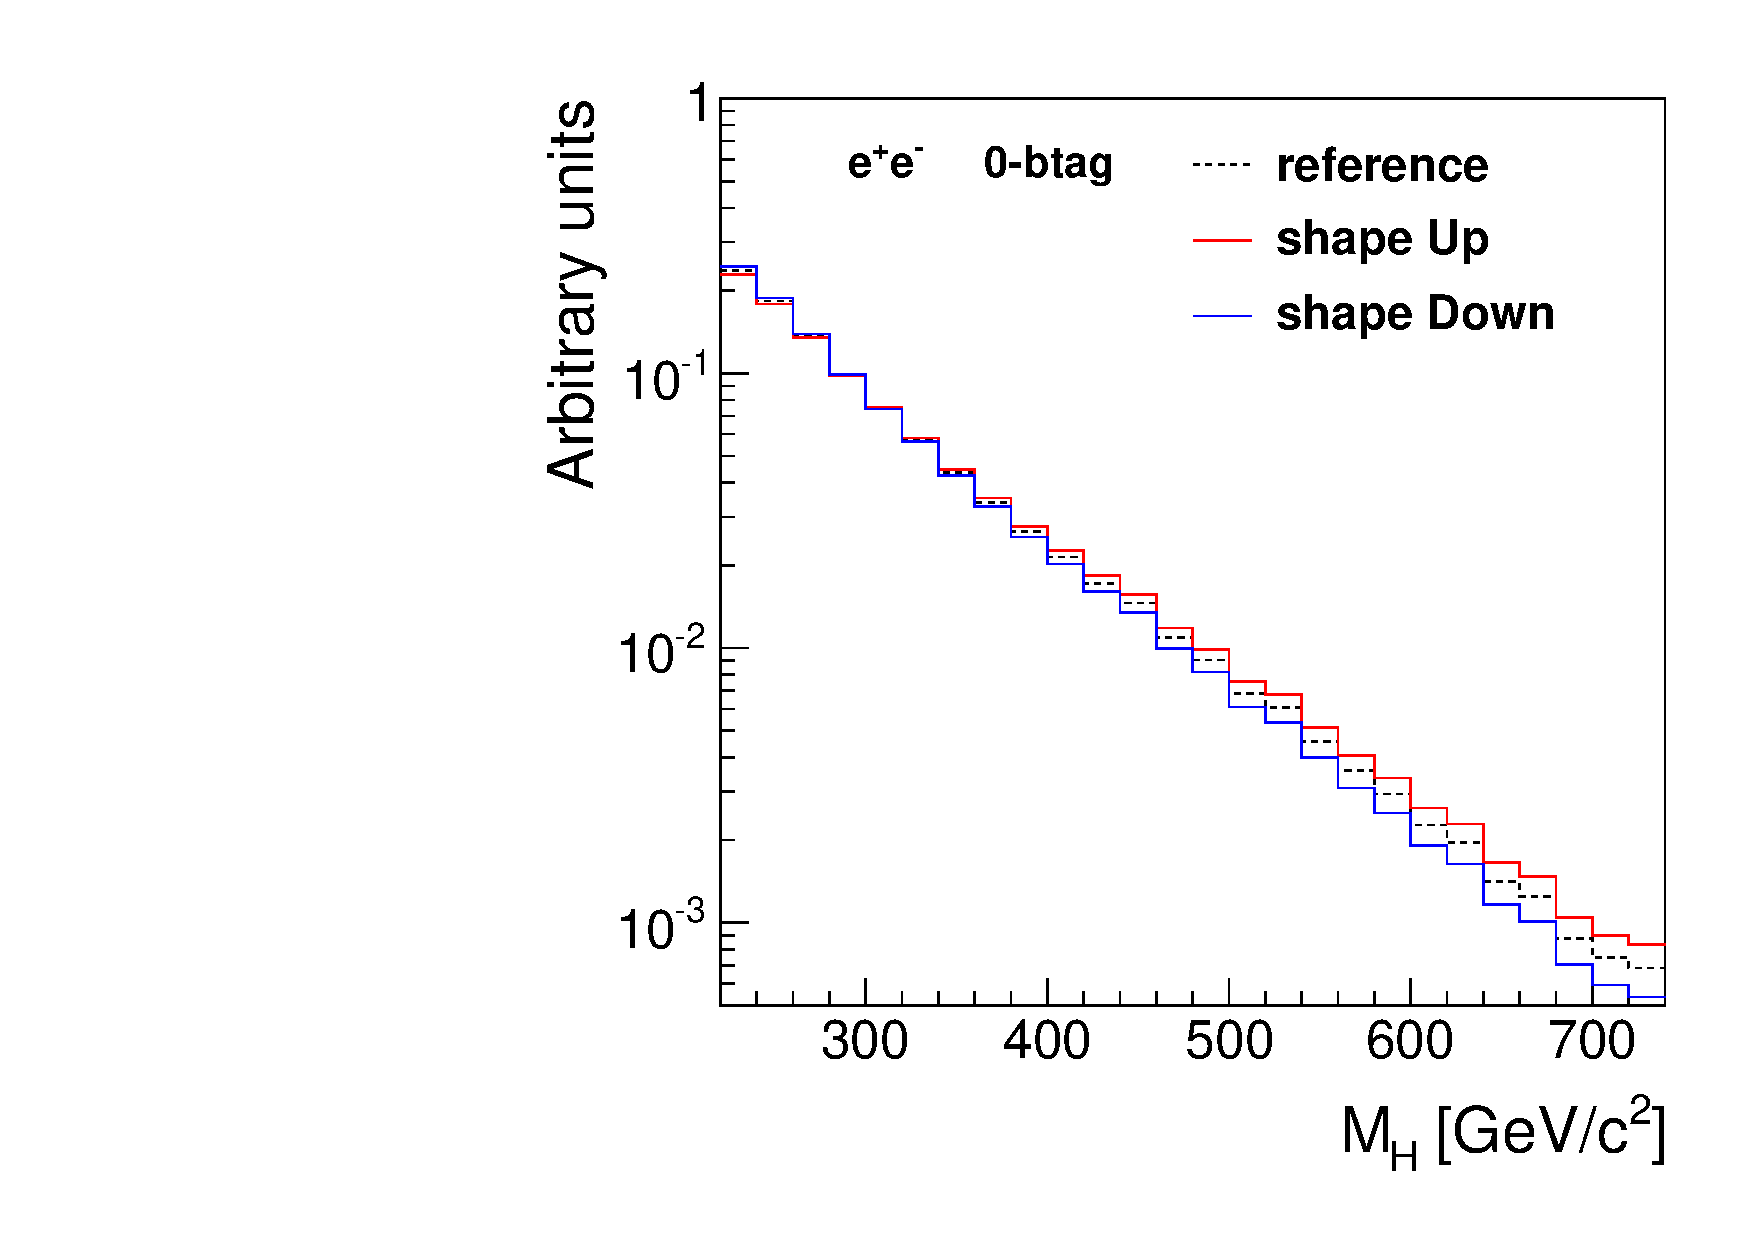
\includegraphics[width=0.33\textwidth]{plots/SBres-ee-0b.pdf}
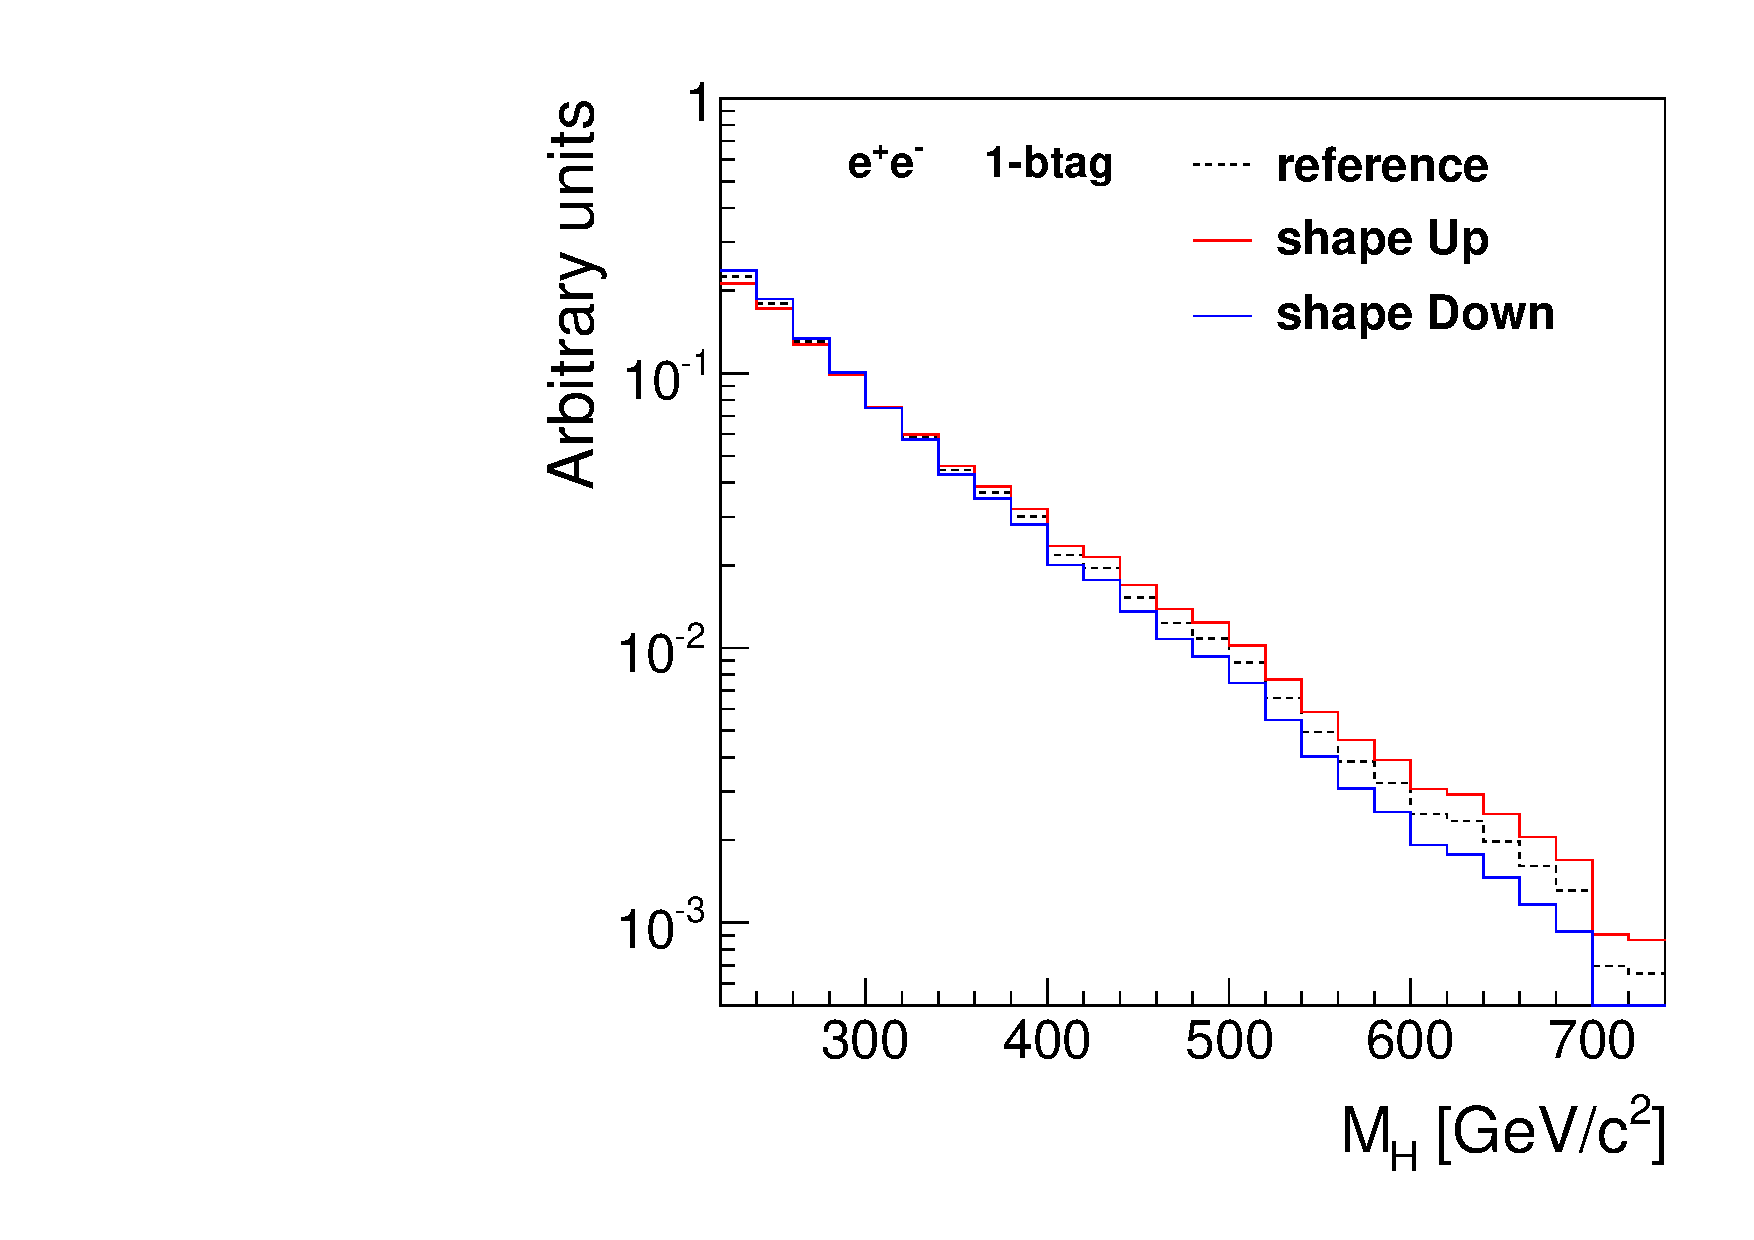
\includegraphics[width=0.33\textwidth]{plots/SBres-ee-1b.pdf}
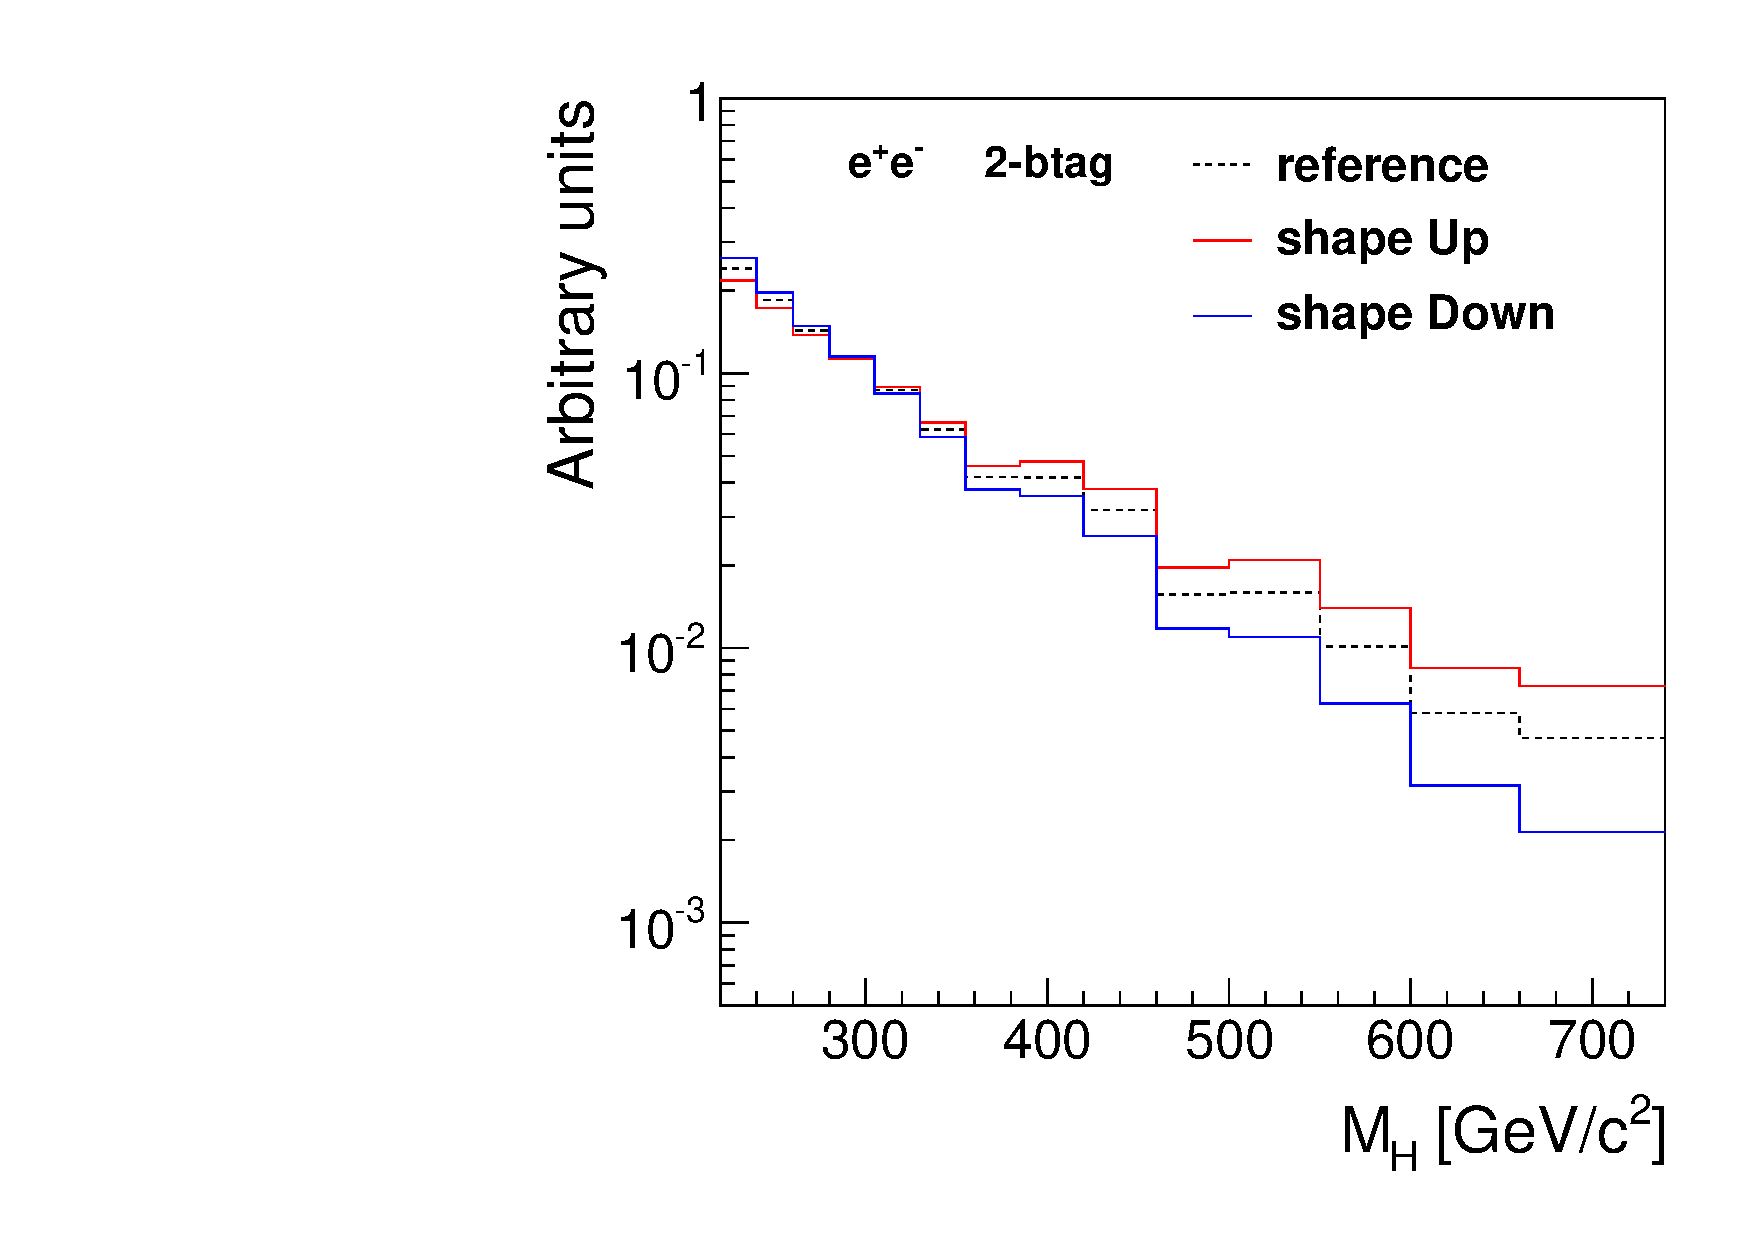
\includegraphics[width=0.33\textwidth]{plots/SBres-ee-2b.pdf}
}
\centerline{
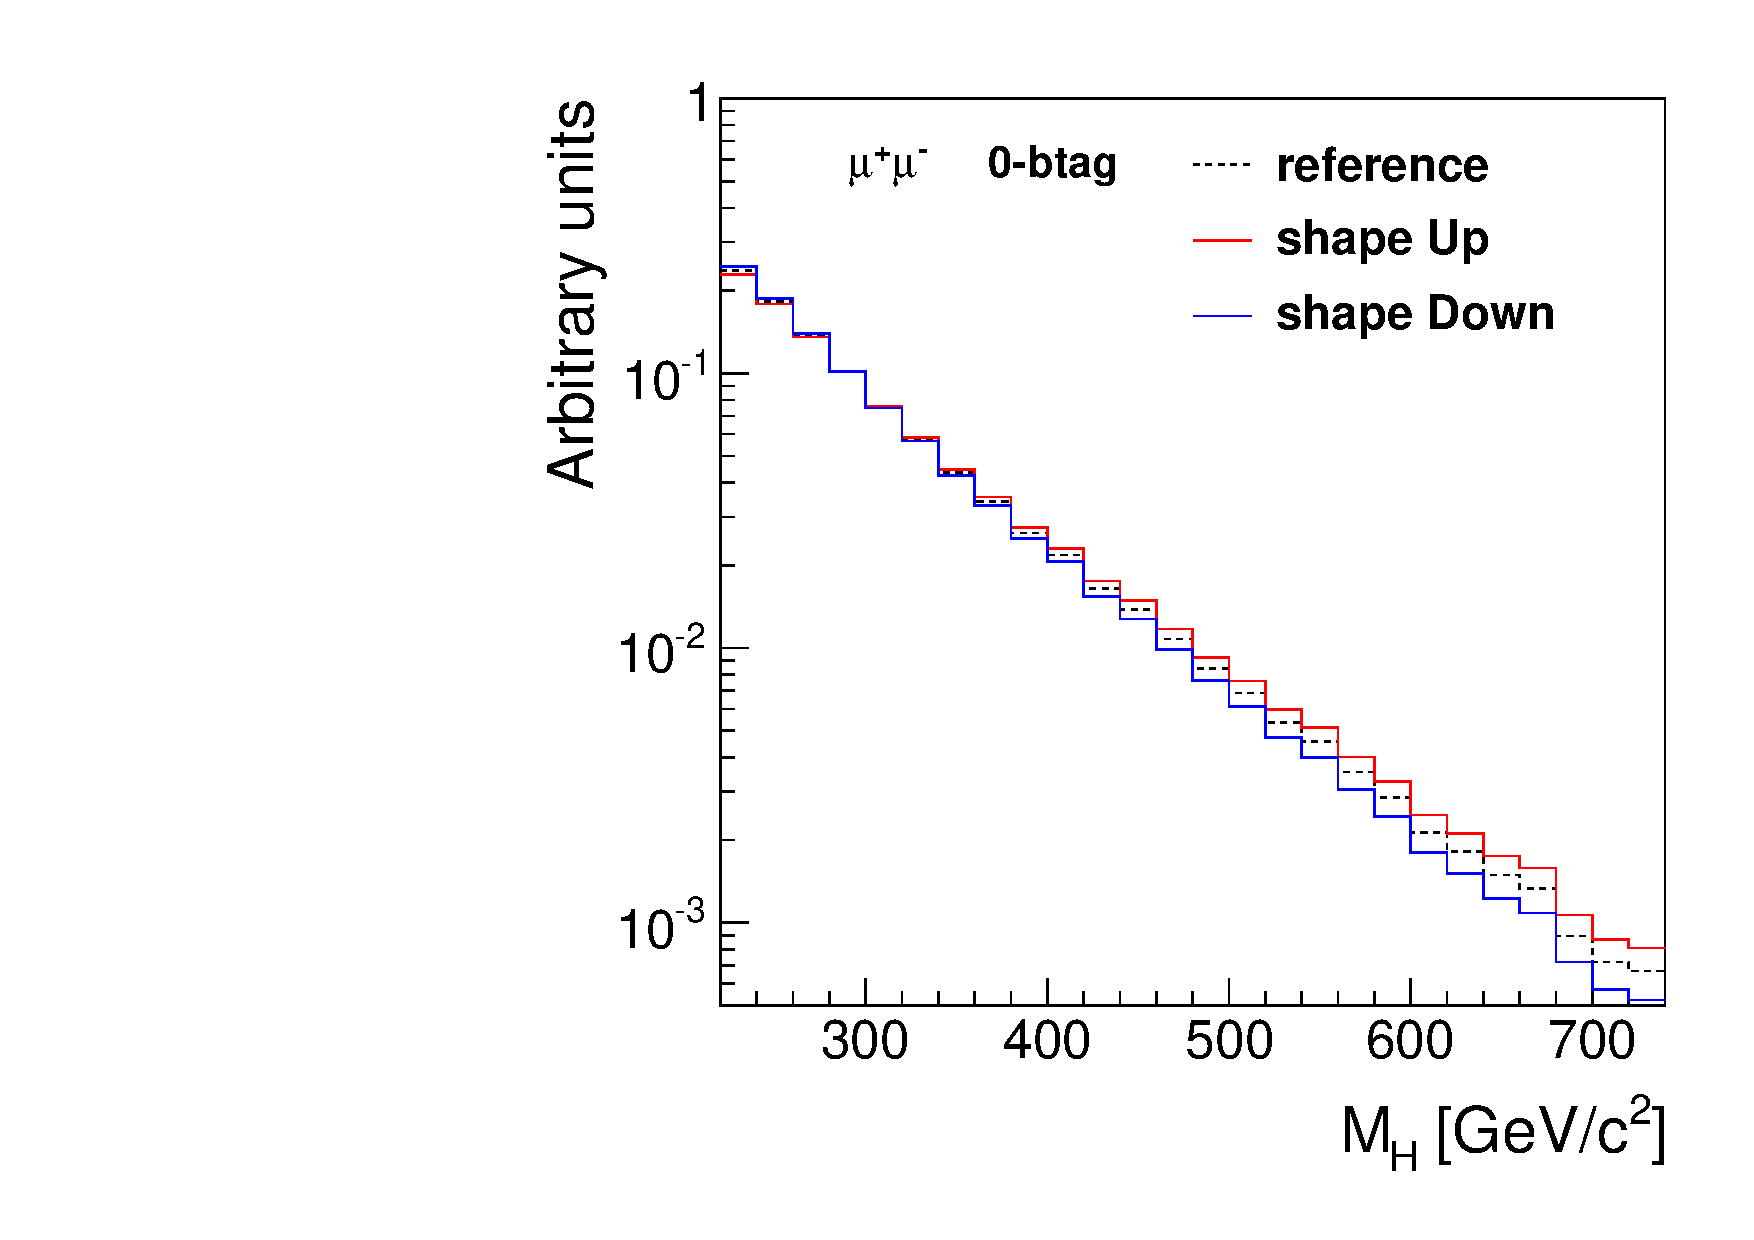
\includegraphics[width=0.33\textwidth]{plots/SBres-mm-0b.pdf}
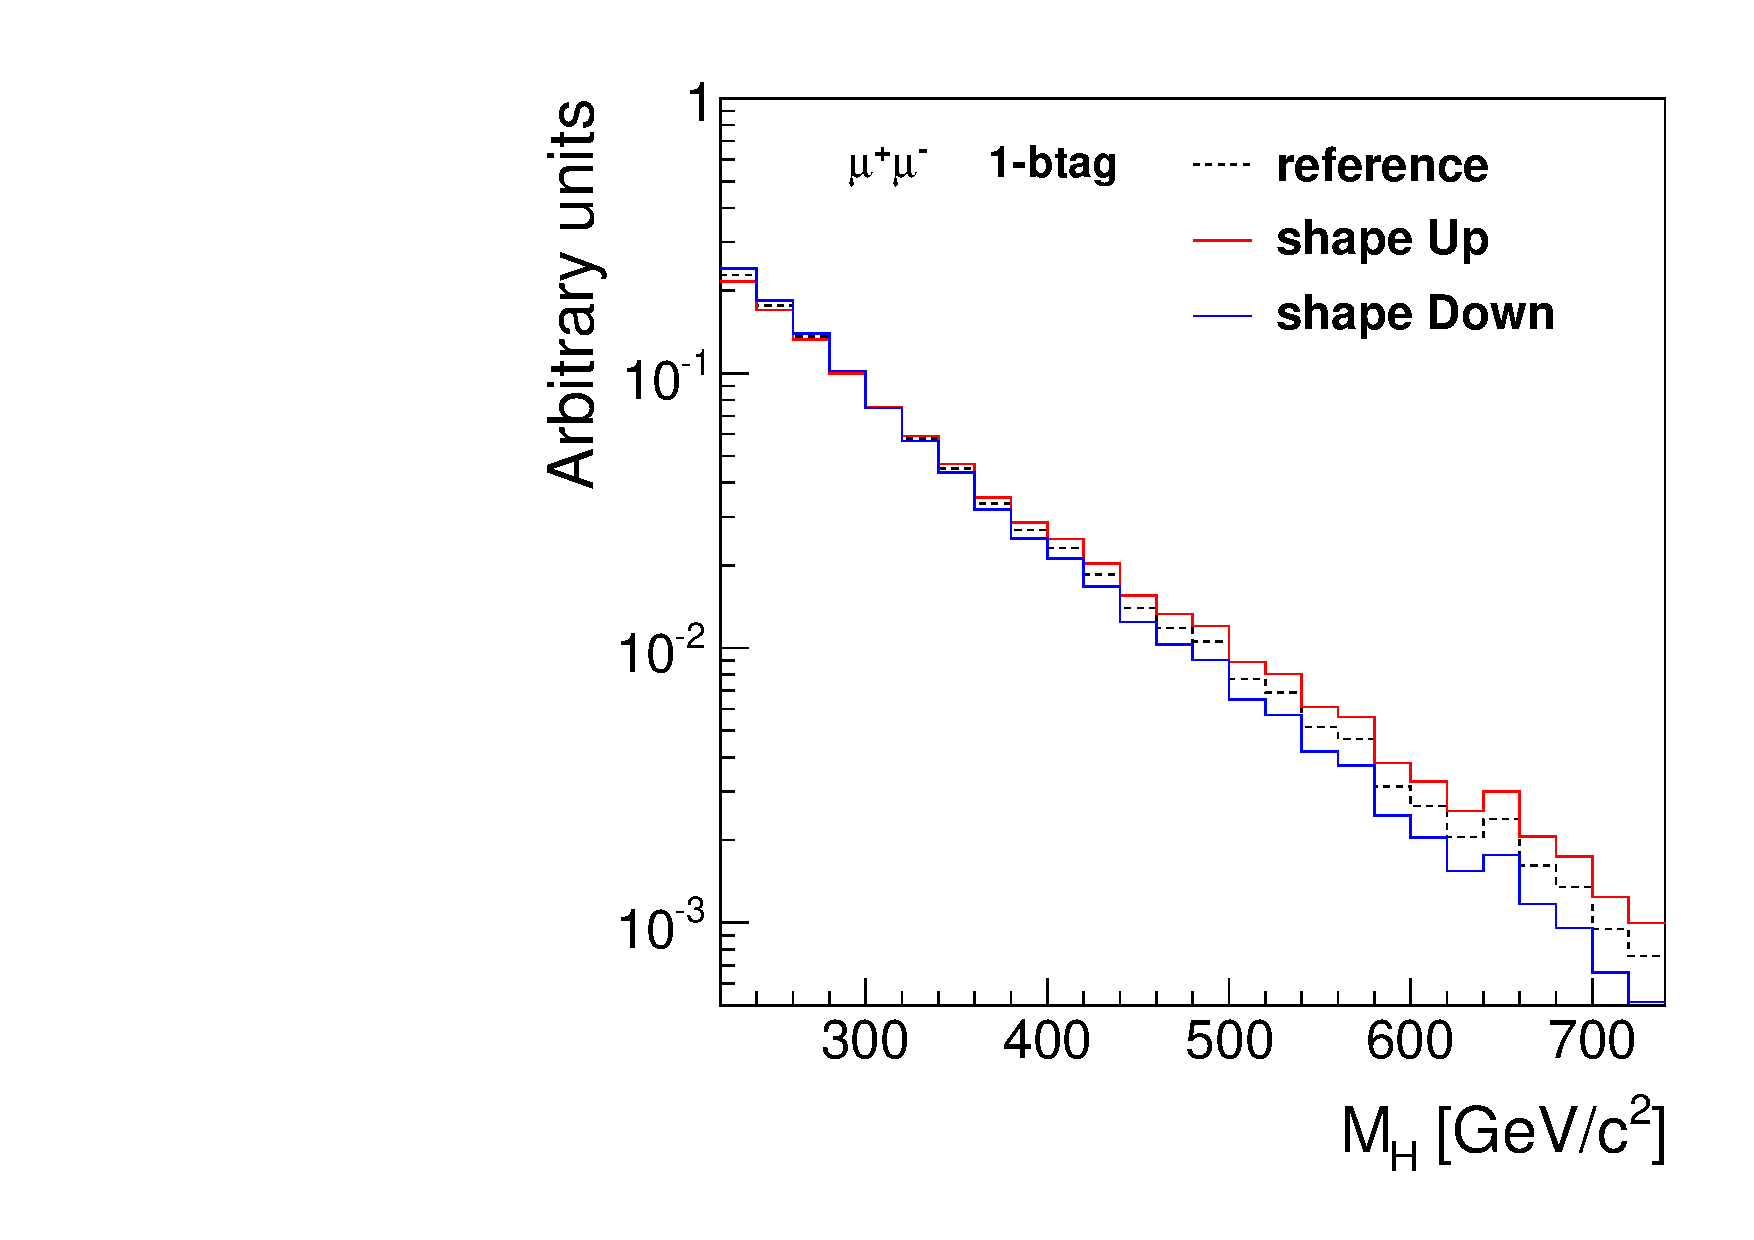
\includegraphics[width=0.33\textwidth]{plots/SBres-mm-1b.pdf}
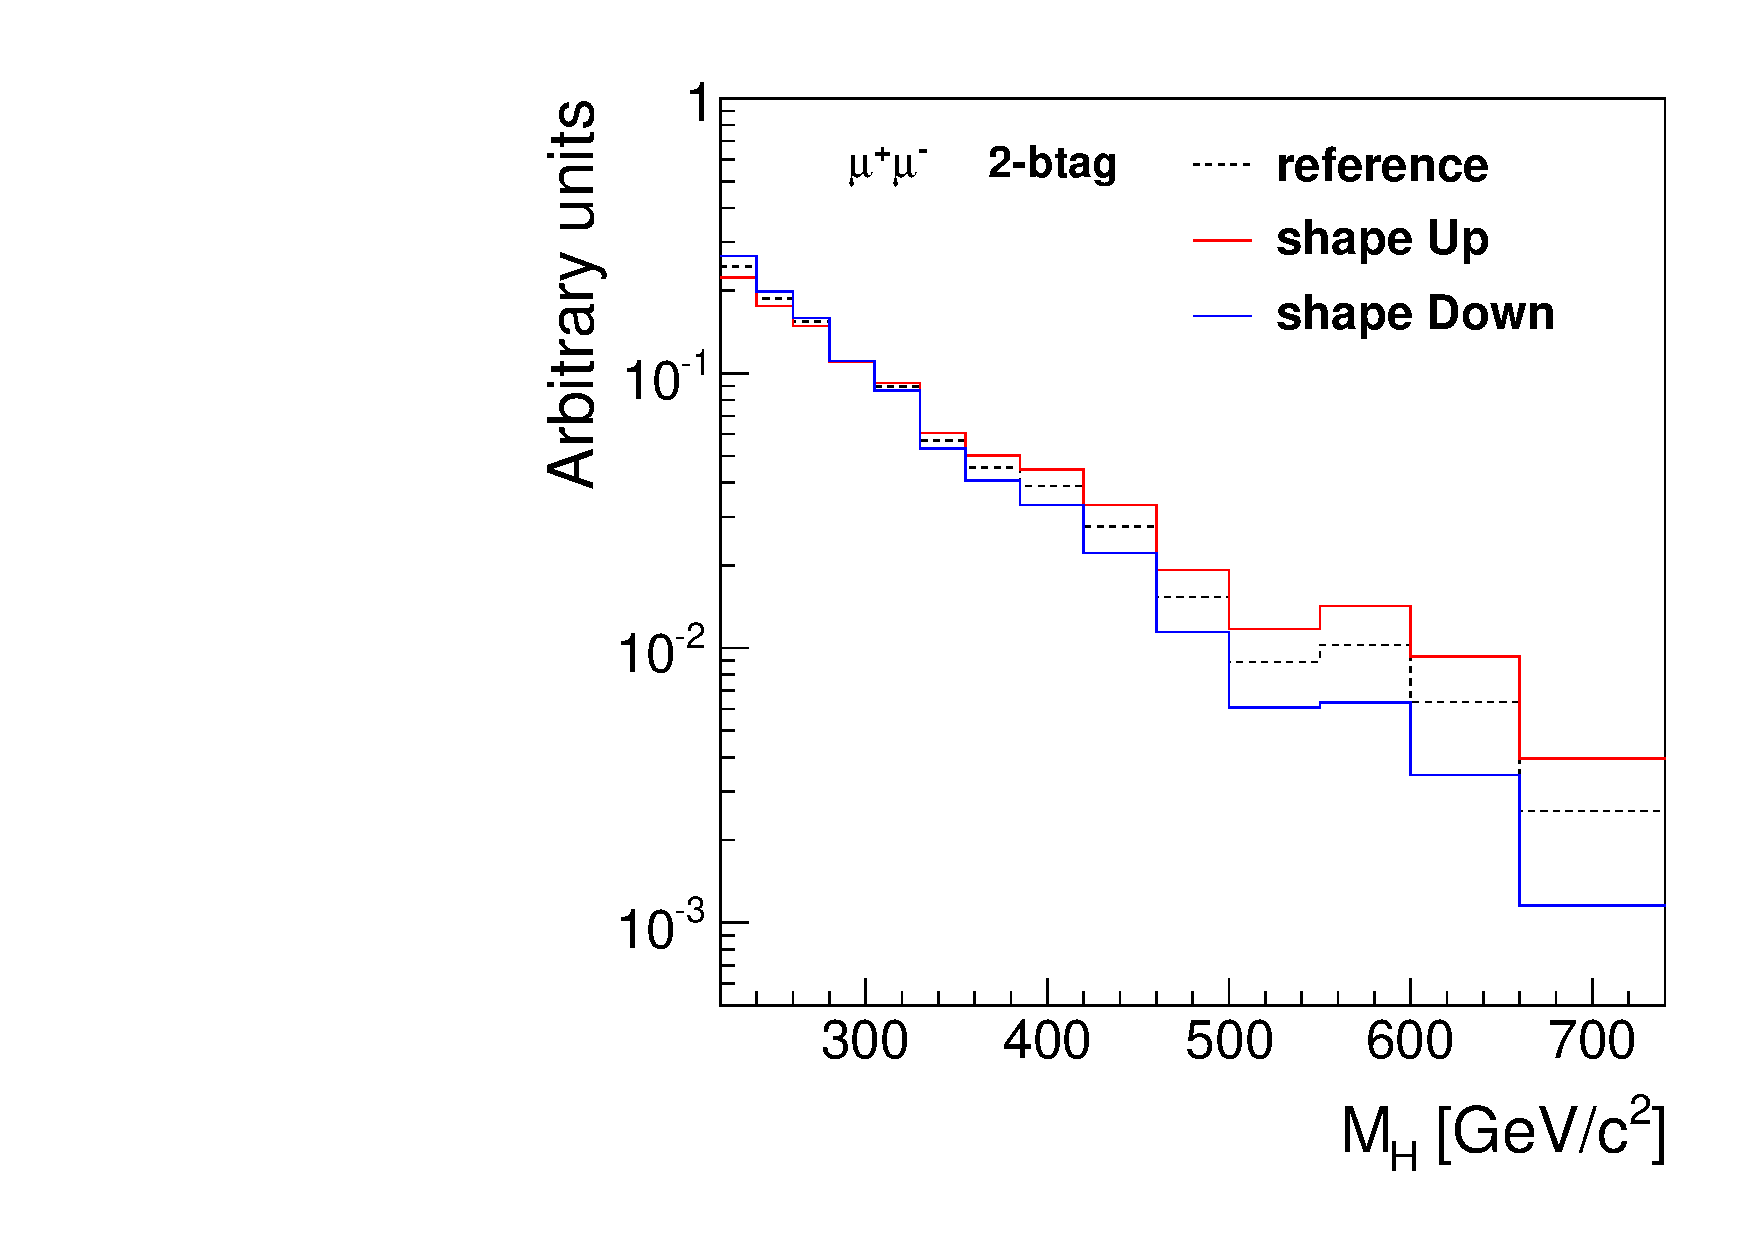
\includegraphics[width=0.33\textwidth]{plots/SBres-mm-2b.pdf}
}
\caption{Residual differences in the $\mlljj$ distributions between the data and the background, in the
$M_{jj}$ sideband control region (top). Alternative templates for the background prediction taking into account those residual variations, for the electron (middle) and the muon channels (bottom).    
}
\label{fig:sysshaperes}
\end{center}
\end{figure}


%%%%%%%%%%%%%%%%%%%%%%%%%%%%%%%%%%%%%%%%%%%%%%%%%%%%%%%%%%%%%%%%%%%%%%%%%%%%%%%%%%%%%%%

\subsection{Upper and Lower Side Band Comparison}

We re-weight the Z+Jets MC in the signal region as seen in Appendix~\ref{sec:emuratios}. In order to estimate how MC reproduced the shape in data for the sideband we plot both data-MC and the ratio $\dfrac{data}{MC}$.  In particular, we also compare the shapes in the lower and upper sidebands to get a more accurate picture of the shape. This gives a more accurate representation of the error in the background than looking at the shape difference between $m_{jjll}$ $p_{T}$ re-weighted and $m_{jjll}$ non $p_{T}$ re-weighted. The exclusive $\PZ$+Jets samples (1-4 jets) are $m_{jjll} p_{T}$ re-weighted.  The data and MC are normalized to unity before comparisons. The plots for all three categories are shown in Figures~\ref{fig:0tag_sideband_up_down},~\ref{fig:1tag_sideband_up_down}, and~\ref{fig:2tag_sideband_up_down}.  

%%%%%%%%%
\begin{figure}[htb!]
%\begin{center}
\centerline{
%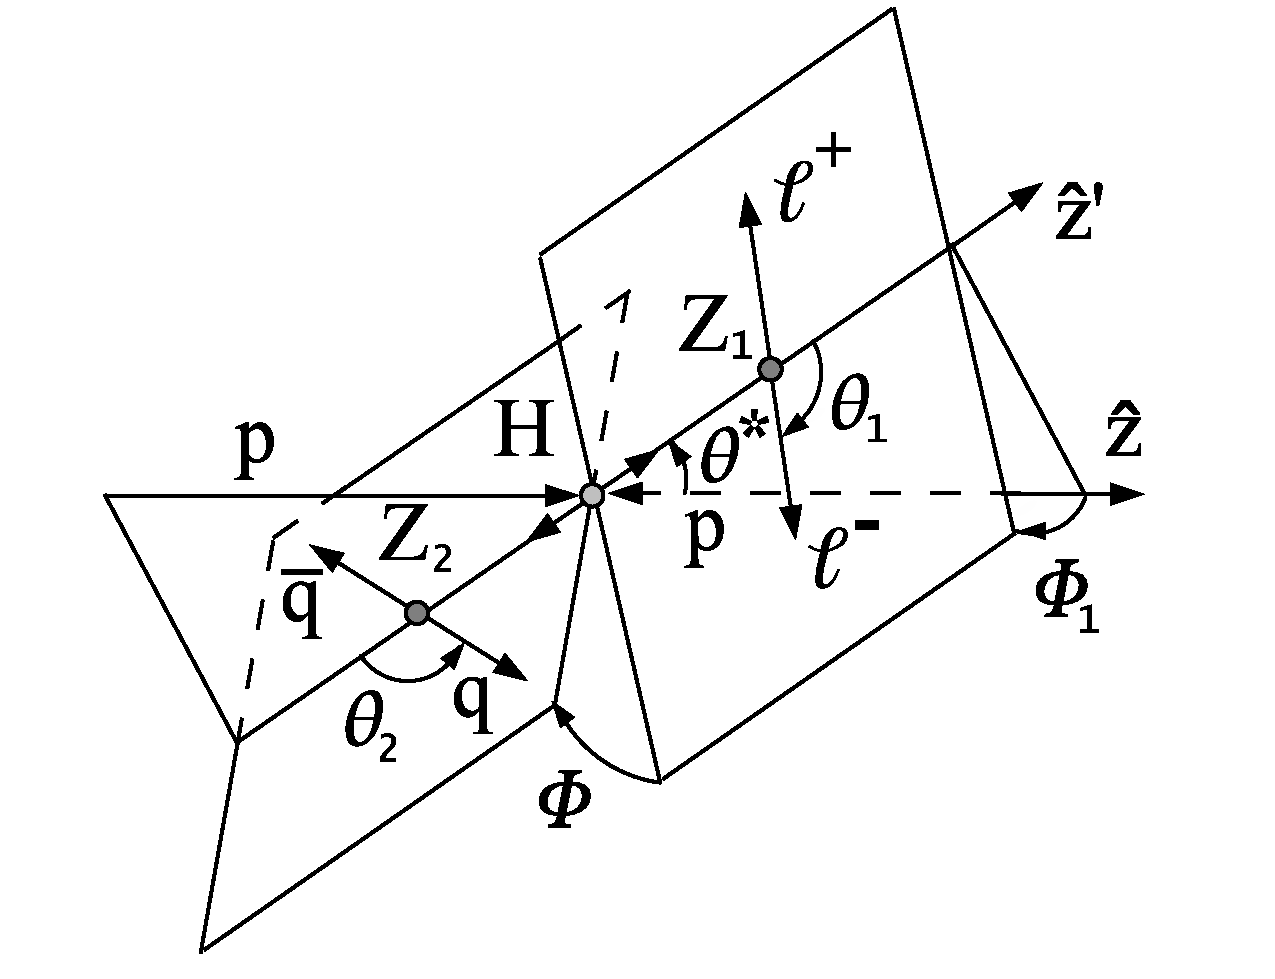
\includegraphics[height=2.5in]{plots/angles-HZZ2l2q}
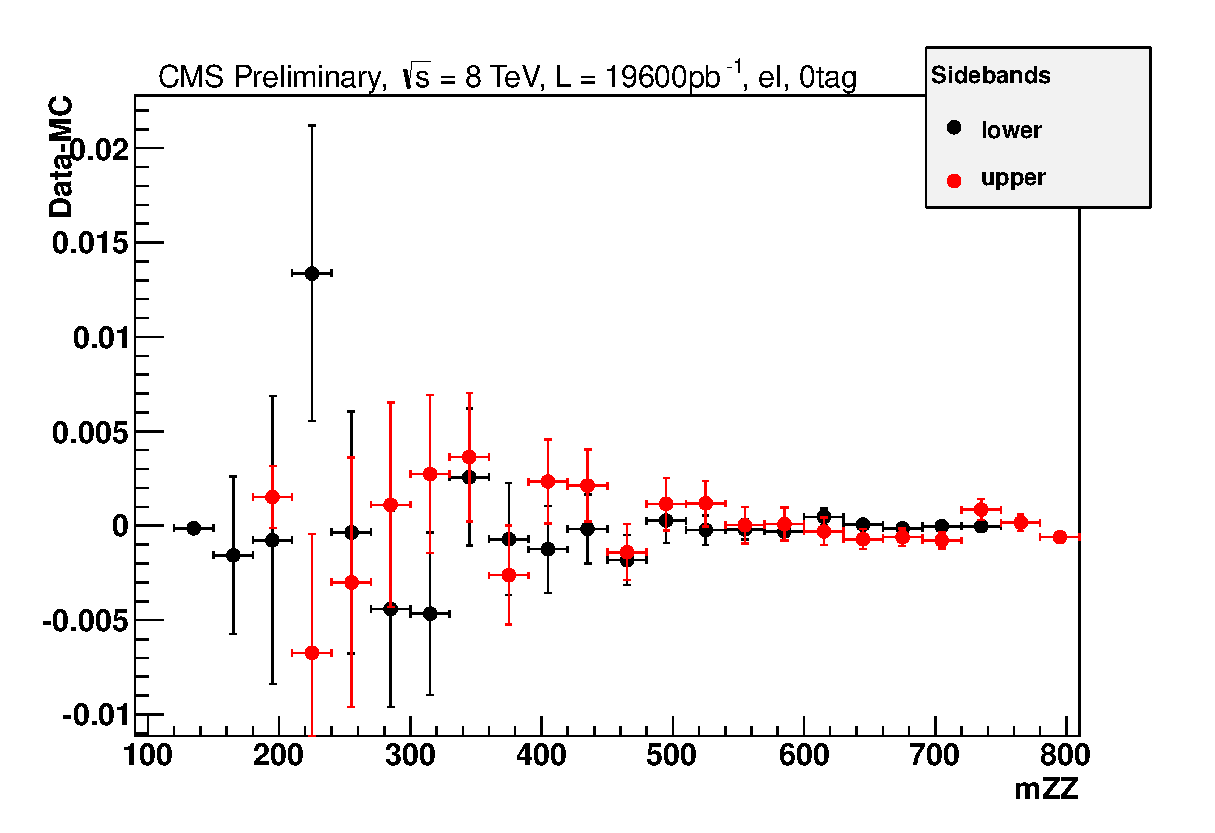
\includegraphics[height=2.5in]{Systematics/plots/subtract_el_2_0}
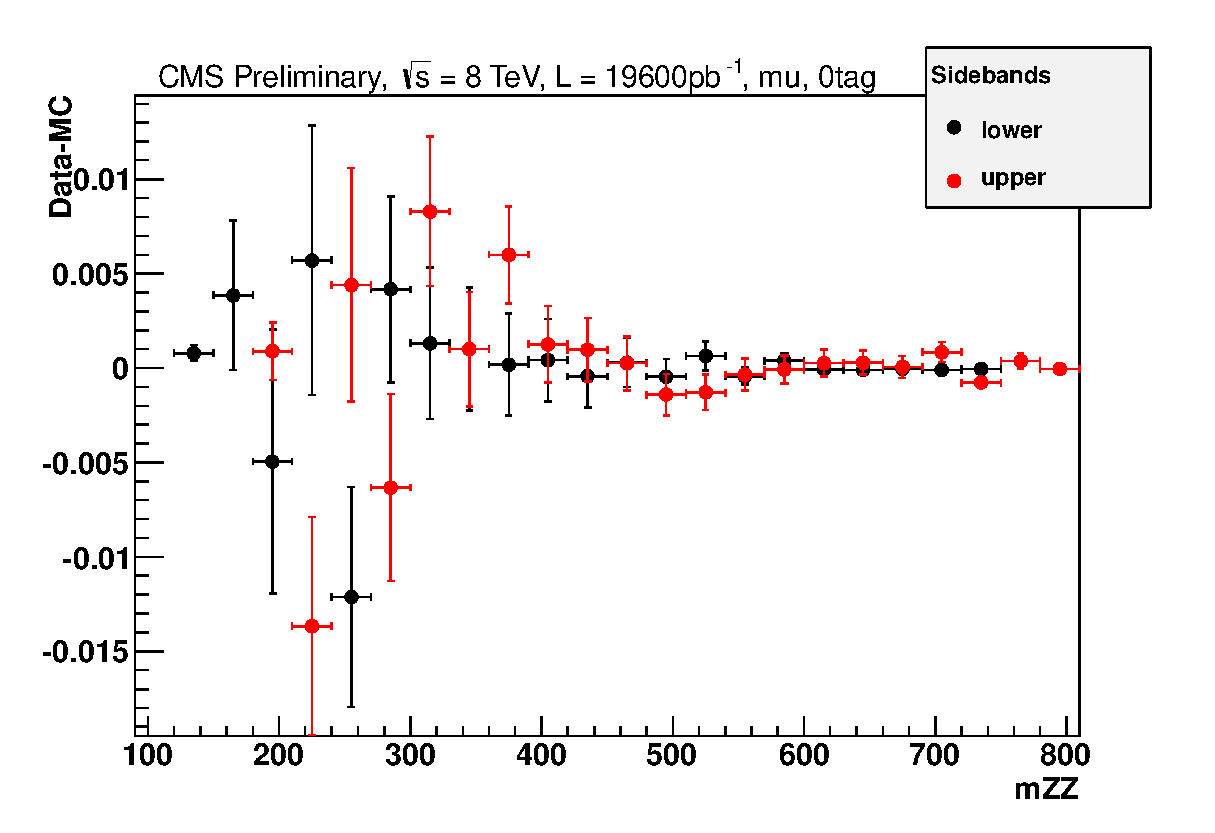
\includegraphics[height=2.5in]{Systematics/plots/subtract_mu_2_0}}
\centerline{
\\
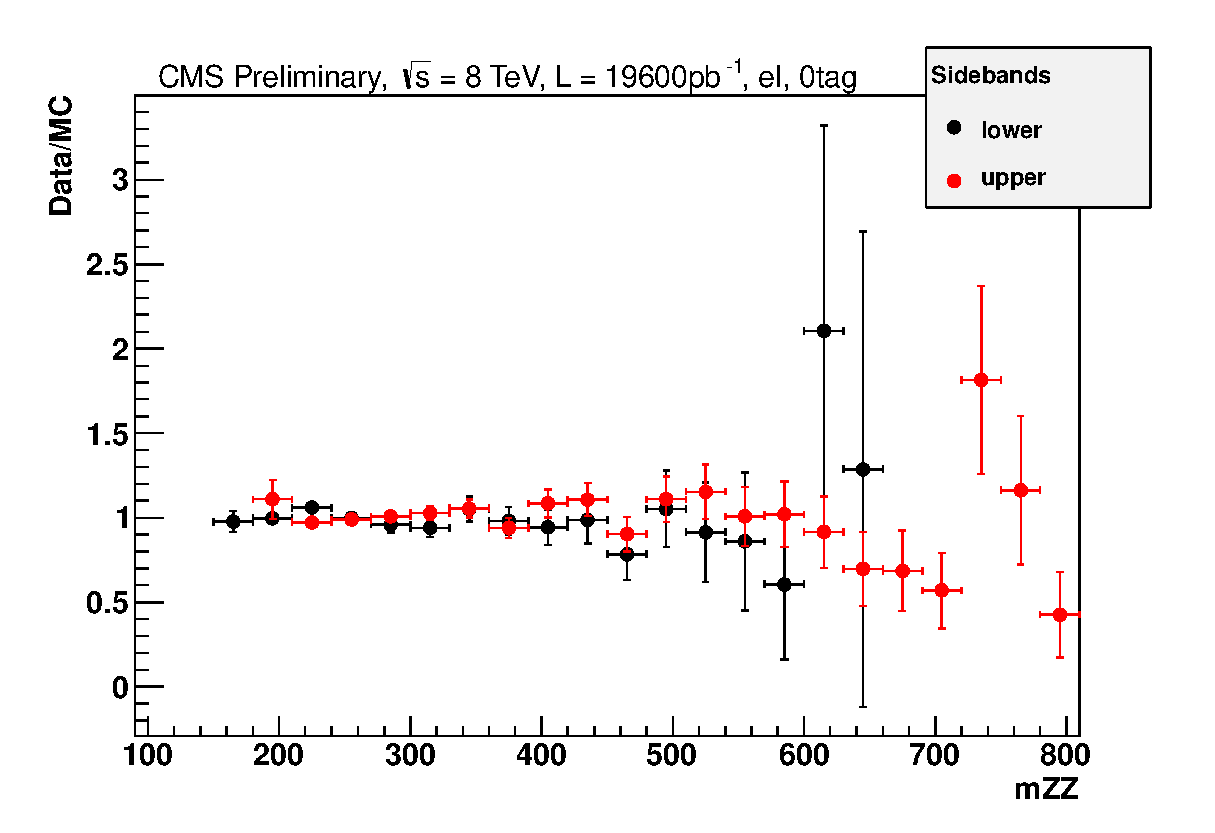
\includegraphics[height=2.5in]{Systematics/plots/divide_el_2_0}
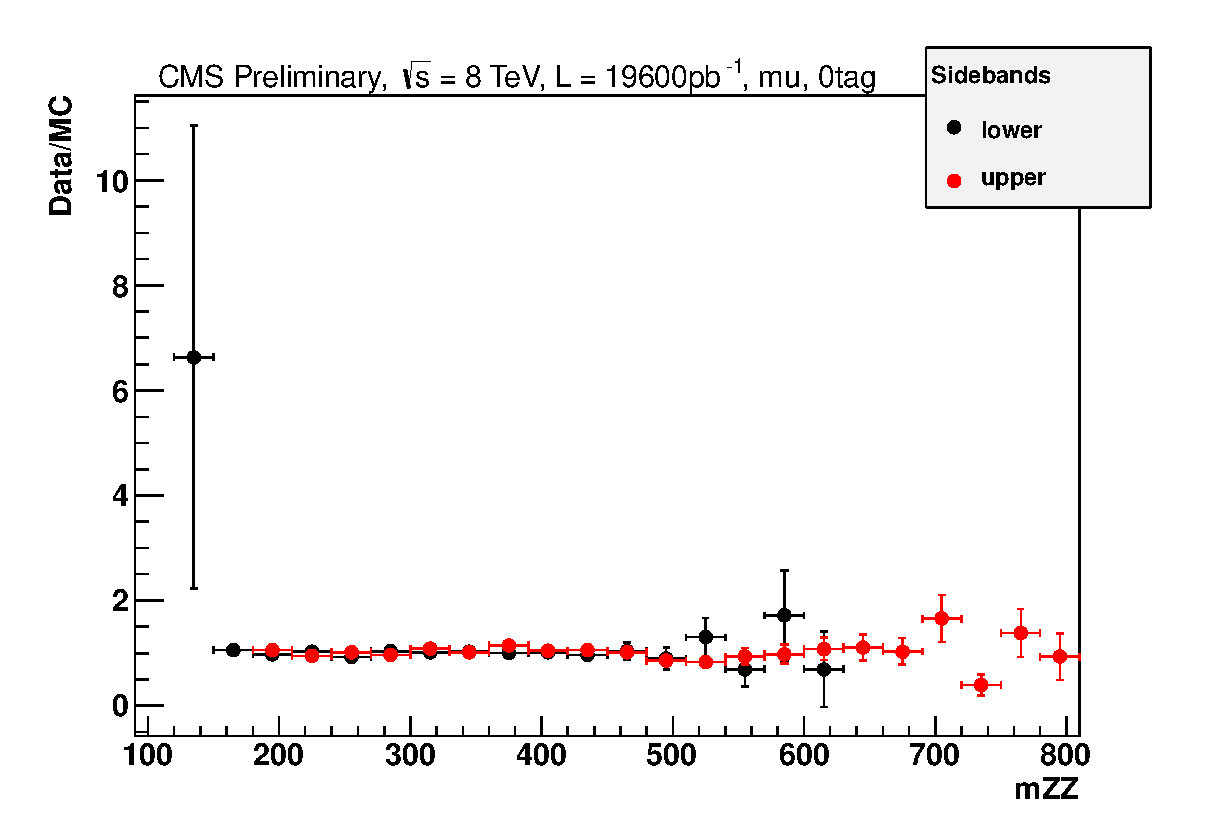
\includegraphics[height=2.5in]{Systematics/plots/divide_mu_2_0}
\\
%\includegraphics[height=2.5in]{plots/angles-Graviton-all2}
}
%\end{center}
\caption{Comparing Data and MC in the 0 btag regions for both the upper sideband and lower sideband regions. Data and MC are first normalized to unity before the comparisons. All plots are a function of the mass of the two Zs. Top left: Data - MC for electrons.  Top right: Data - MC for muons.  Bottom left: Data/MC for electrons.  Bottom right: Data/MC for muons.
\label{fig:0tag_sideband_up_down}}  
\end{figure}
%%%%%%%%%
\begin{figure}[htb!]
%\begin{center}
\centerline{
%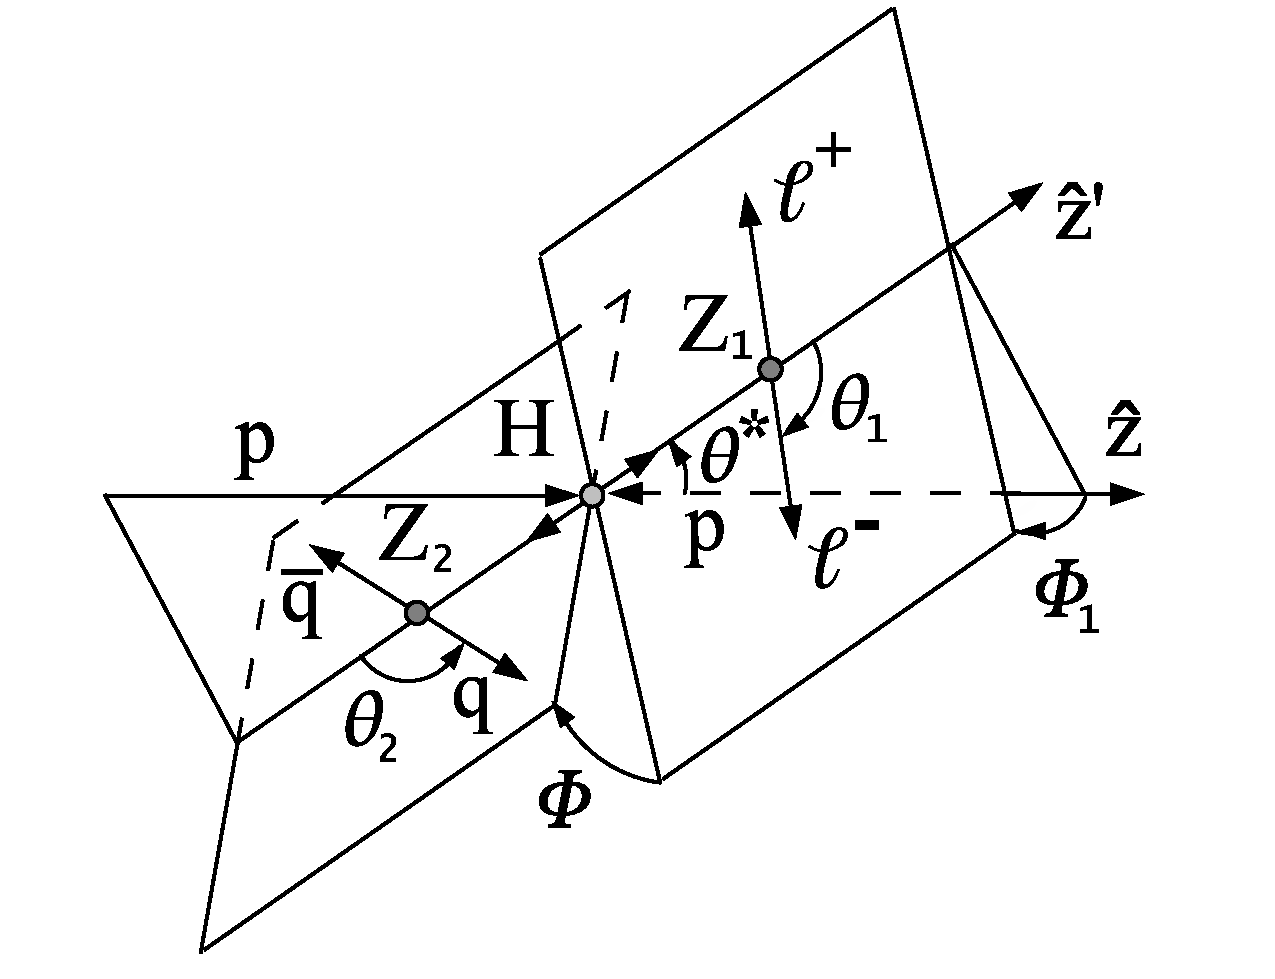
\includegraphics[height=2.5in]{plots/angles-HZZ2l2q}
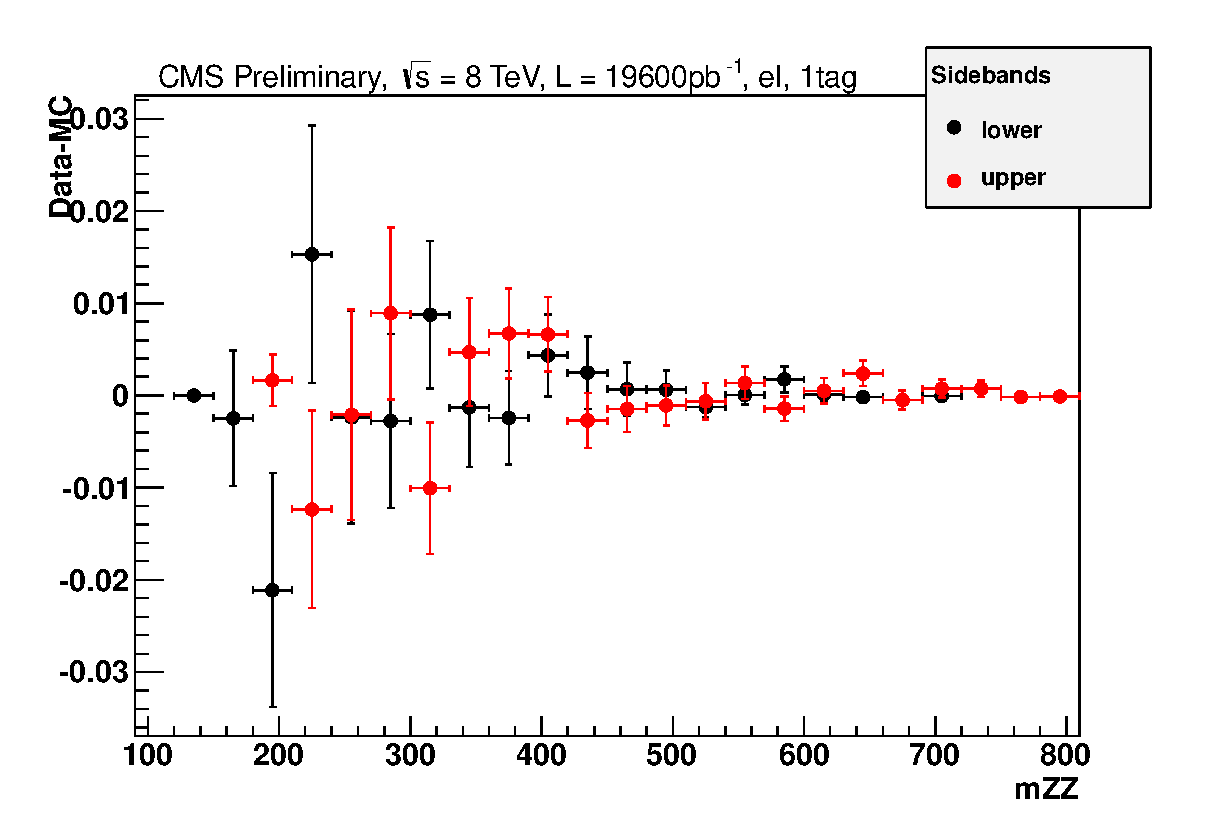
\includegraphics[height=2.5in]{Systematics/plots/subtract_el_2_1}
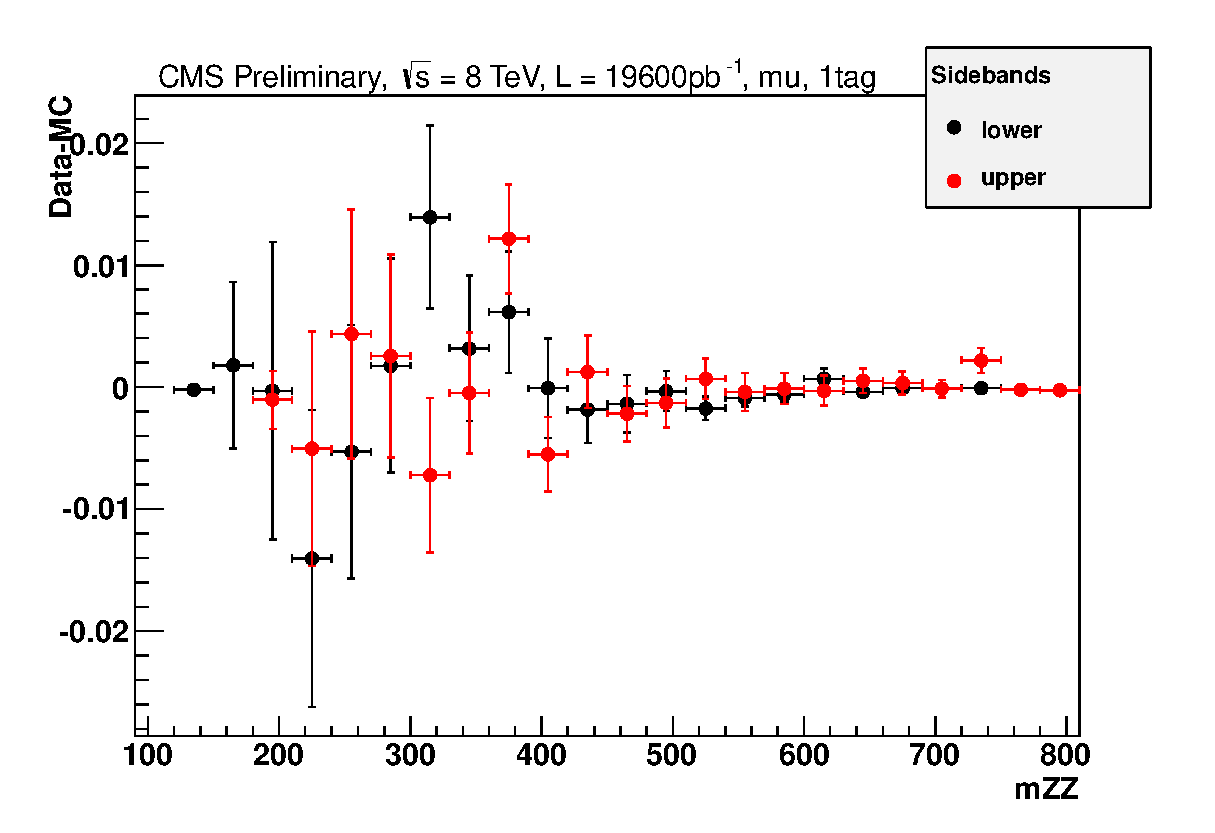
\includegraphics[height=2.5in]{Systematics/plots/subtract_mu_2_1}}
\centerline{
\\
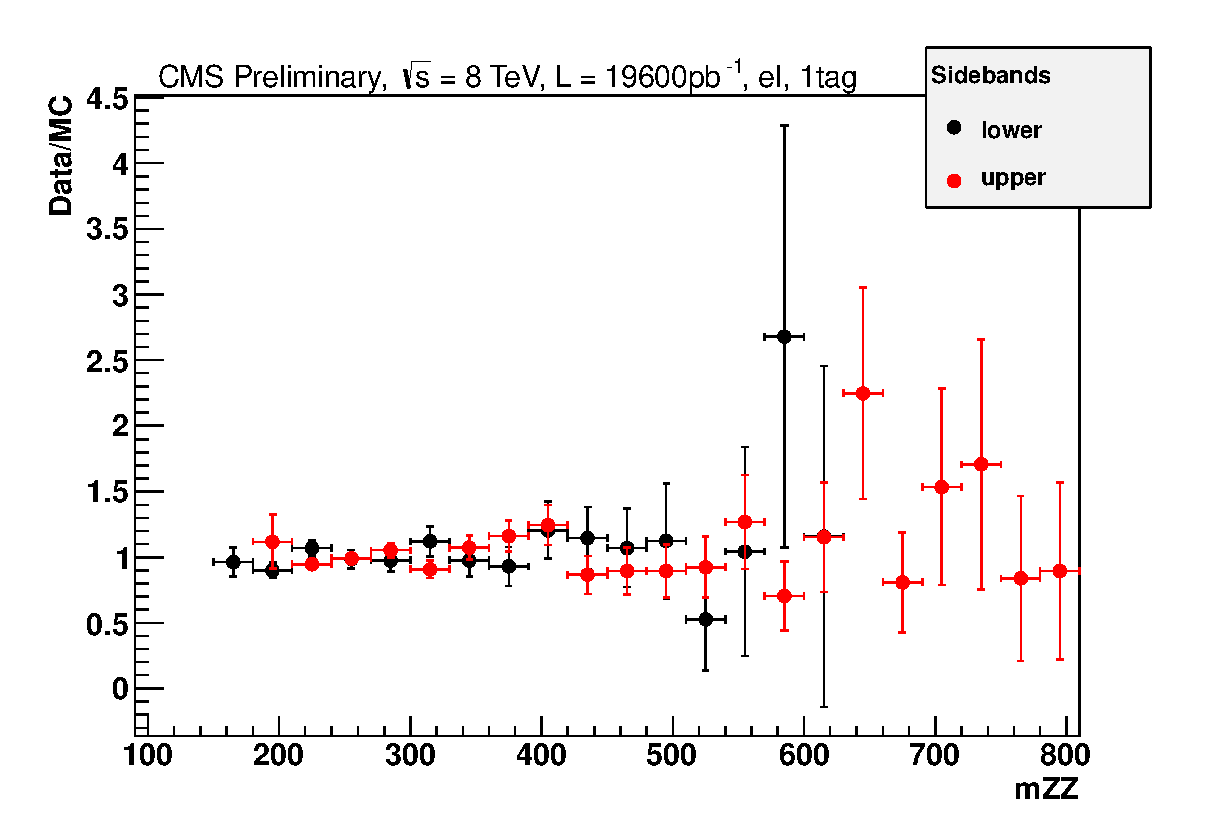
\includegraphics[height=2.5in]{Systematics/plots/divide_el_2_1}
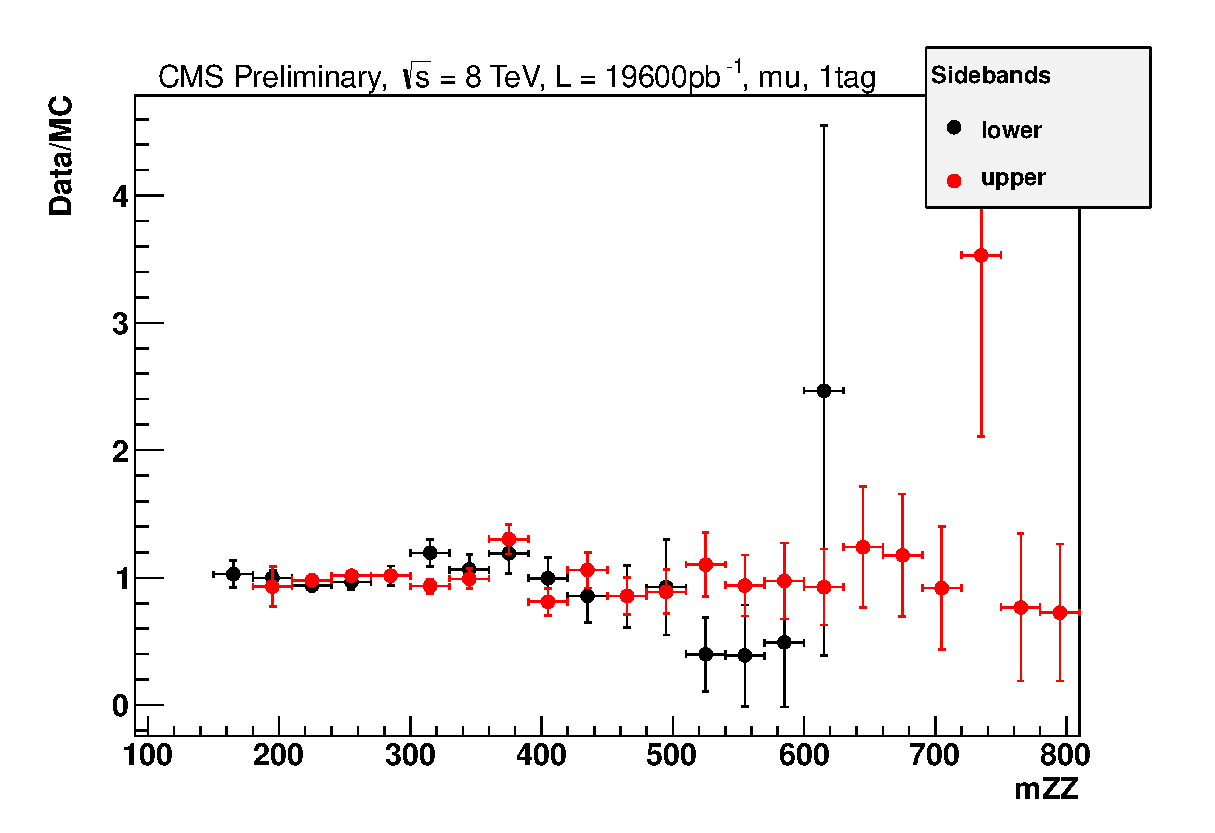
\includegraphics[height=2.5in]{Systematics/plots/divide_mu_2_1}
\\
%\includegraphics[height=2.5in]{plots/angles-Graviton-all2}
}
%\end{center}
\caption{Comparing Data and MC in the 1 btag regions for both the upper sideband and lower sideband regions. Data and MC are first normalized to unity before the comparisons. All plots are a function of the mass of the two Zs. Top left: Data - MC for electrons.  Top right: Data - MC for muons.  Bottom left: Data/MC for electrons.  Bottom right: Data/MC for muons.
\label{fig:1tag_sideband_up_down}}  
\end{figure}
%%%%%%%%%
\begin{figure}[htb!]
%\begin{center}
\centerline{
%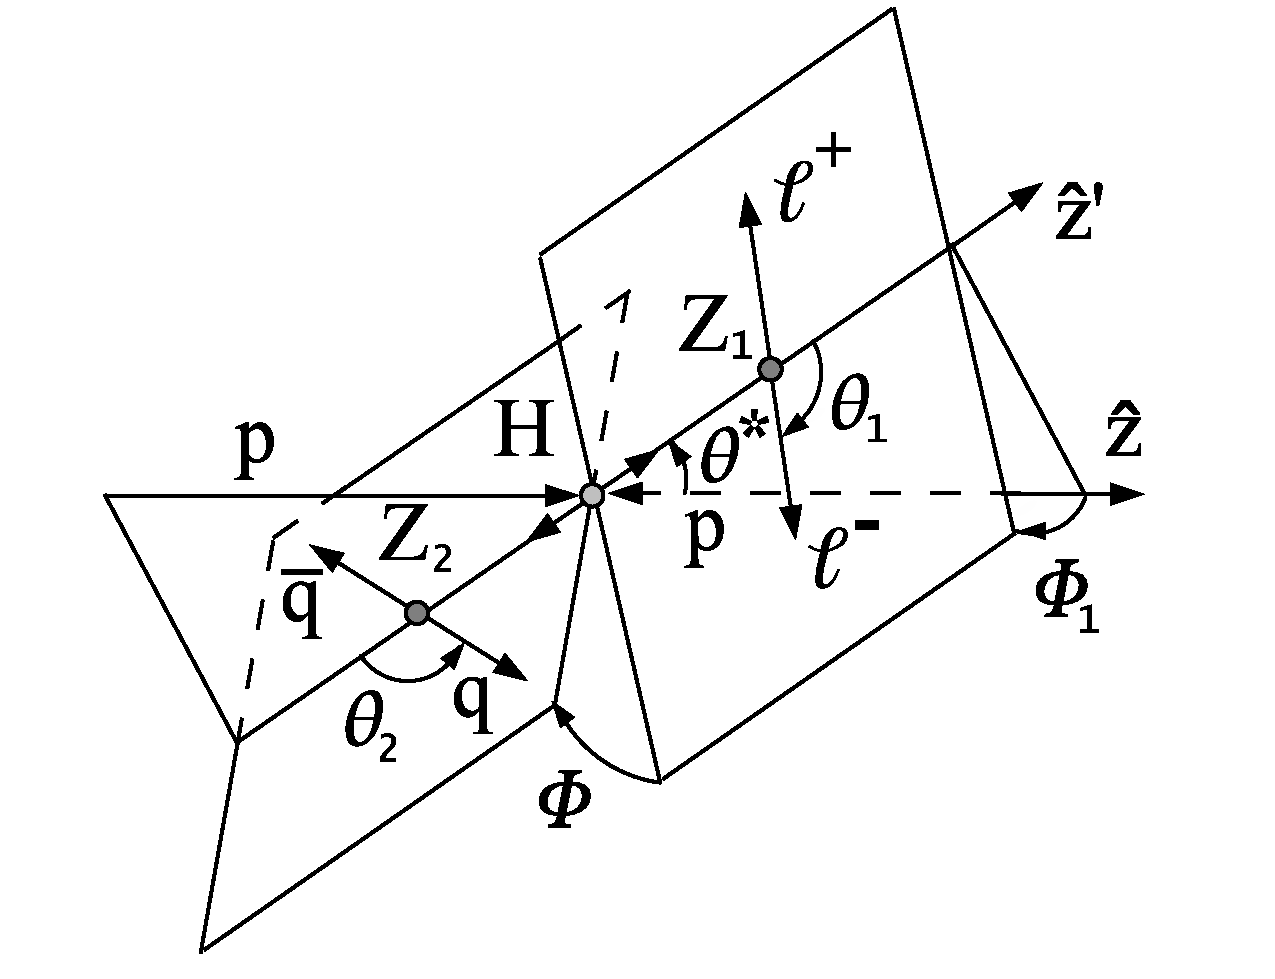
\includegraphics[height=2.5in]{plots/angles-HZZ2l2q}
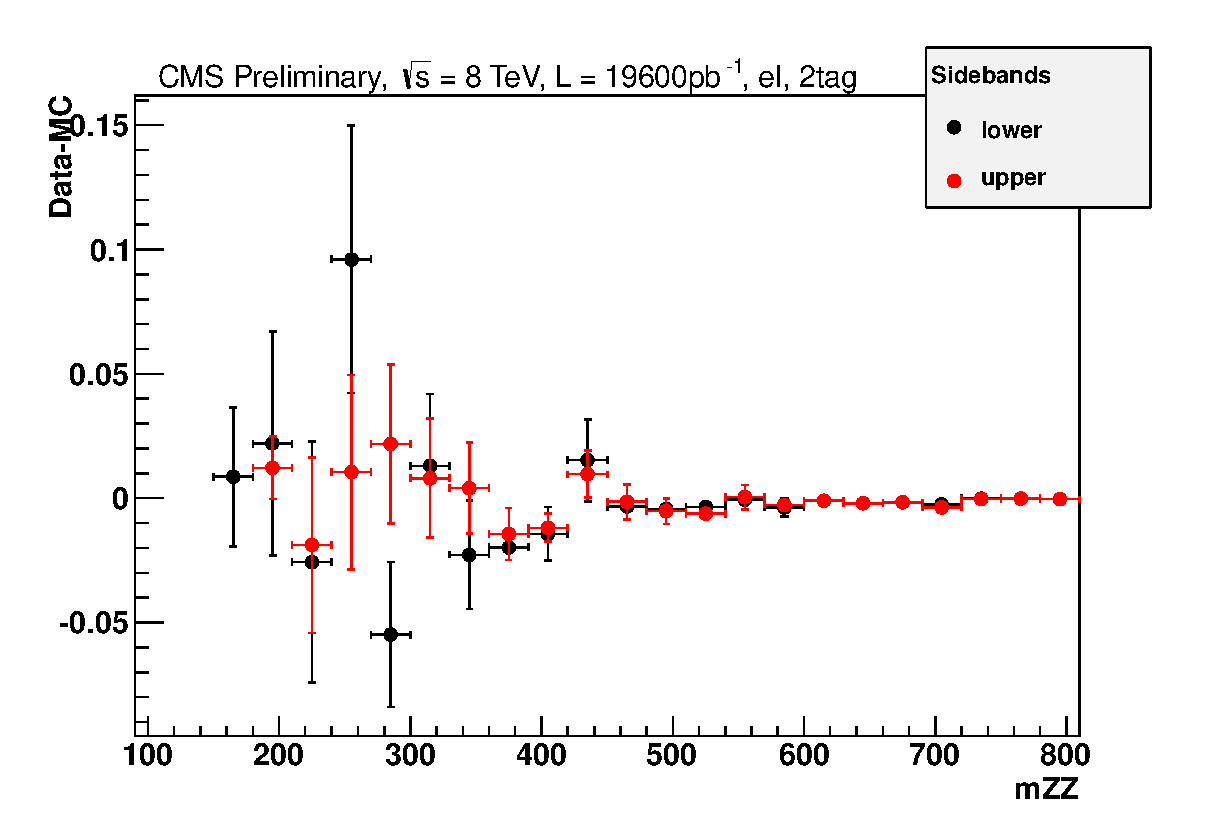
\includegraphics[height=2.5in]{Systematics/plots/subtract_el_2_2}
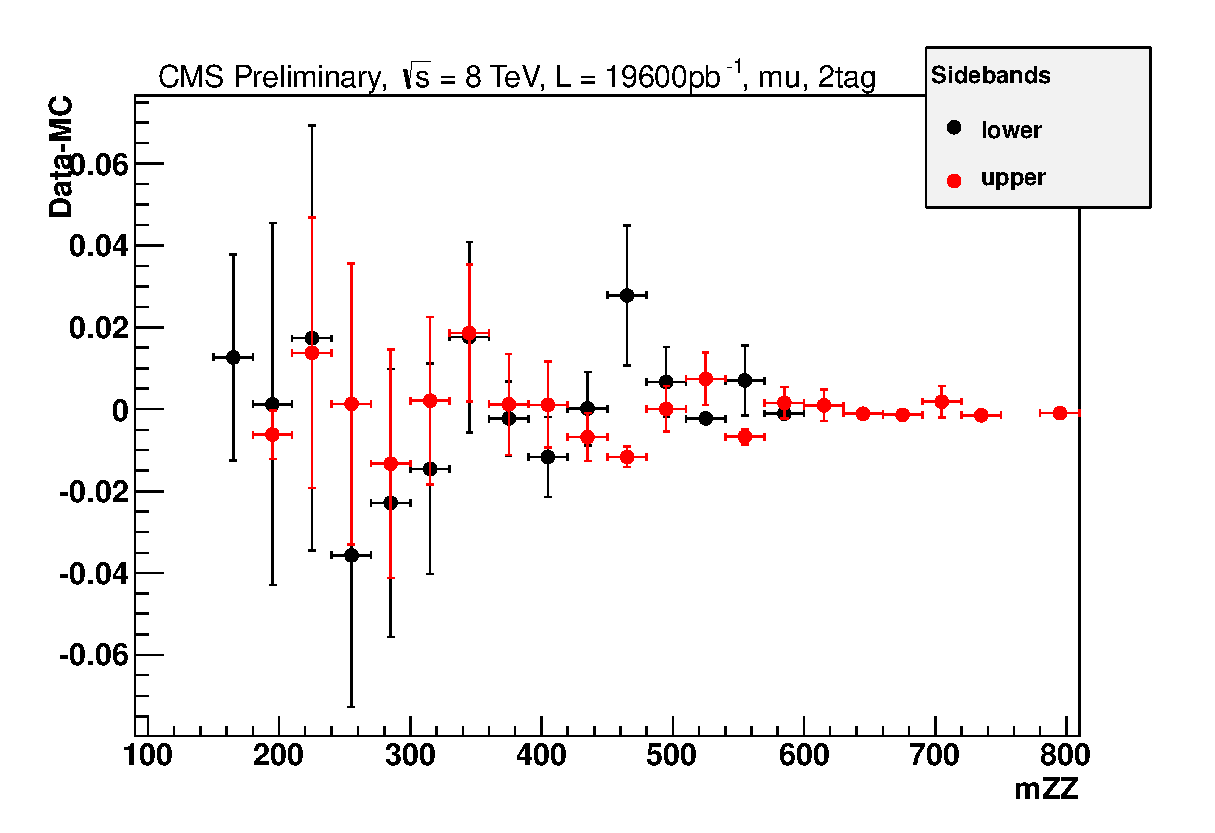
\includegraphics[height=2.5in]{Systematics/plots/subtract_mu_2_2}}
\centerline{
\\
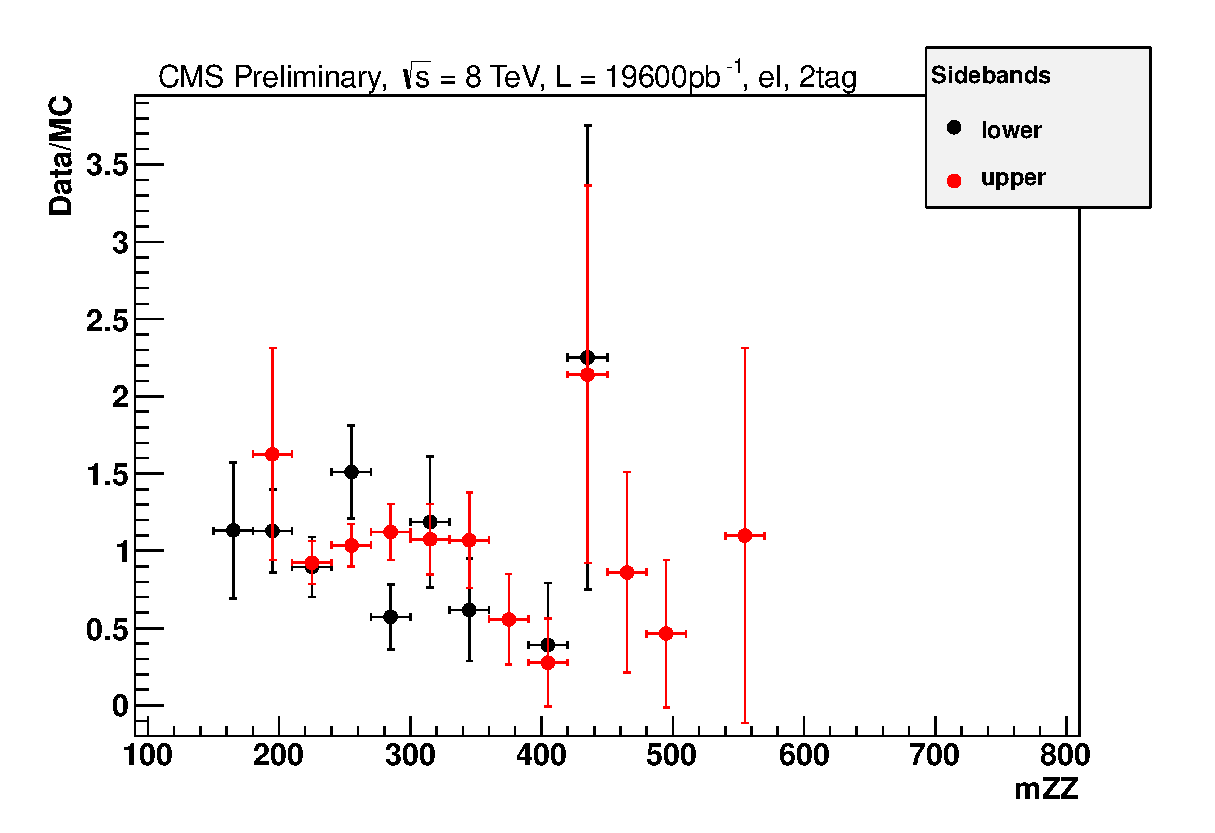
\includegraphics[height=2.5in]{Systematics/plots/divide_el_2_2}
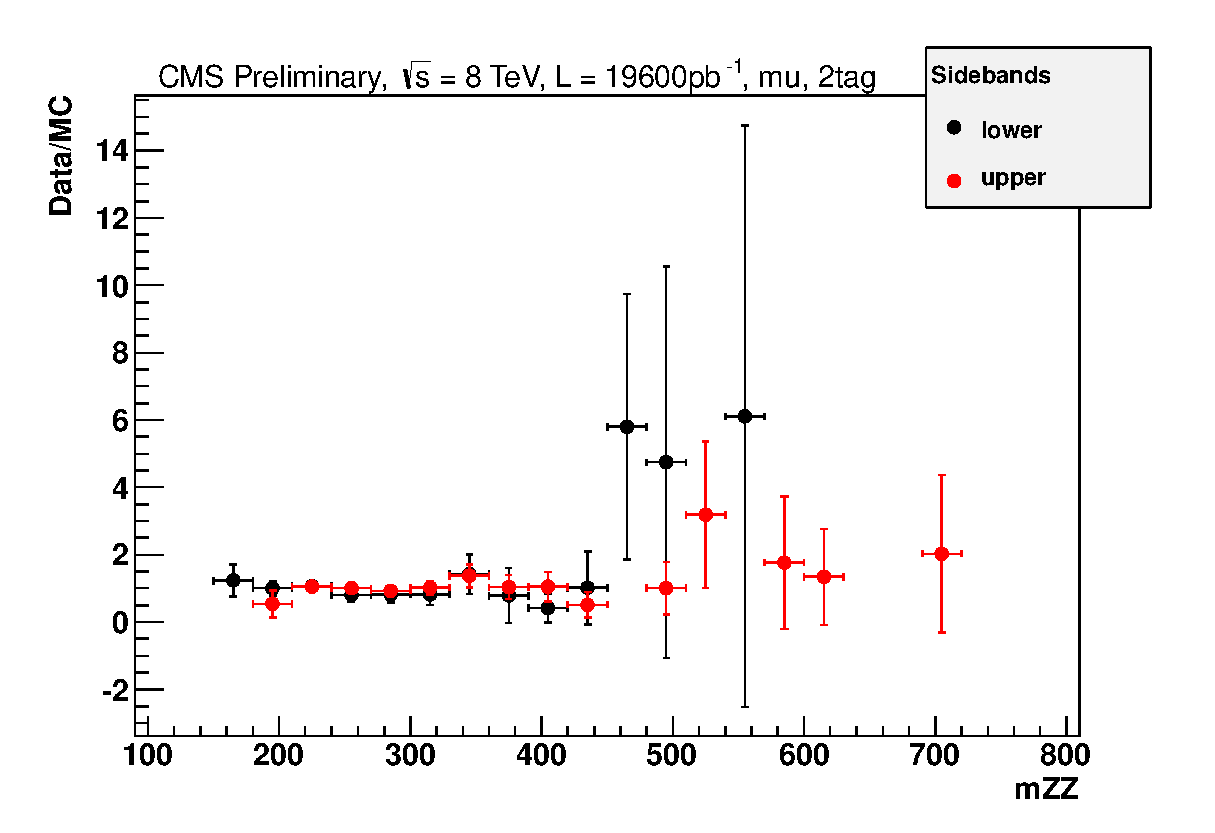
\includegraphics[height=2.5in]{Systematics/plots/divide_mu_2_2}
\\
%\includegraphics[height=2.5in]{plots/angles-Graviton-all2}
}
%\end{center}
\caption{Comparing Data and MC in the 2 btag regions for both the upper sideband and lower sideband regions. Data and MC are first normalized to unity before the comparisons. All plots are a function of the mass of the two Zs. Top left: Data - MC for electrons.  Top right: Data - MC for muons.  Bottom left: Data/MC for electrons.  Bottom right: Data/MC for muons.
\label{fig:2tag_sideband_up_down}}  
\end{figure}
%%%%%%%%%




%\subsection{Subsection heading}

%\subsubsection{Subsubsection heading}

